
% Build with pdfLaTeX and BibTeX, for example on Overleaf (set main.tex as the main document) or with
%   pdflatex main && bibtex main && pdflatex main && pdflatex main
% Generated by build_tex.py from paper/PAPER.md; edit PAPER.md or build_tex.py and rebuild rather than
% editing the chapter files by hand, or the next build will overwrite the edit.
\documentclass[12pt,a4paper,oneside]{report}
\usepackage[T1]{fontenc}
\usepackage[utf8]{inputenc}
\usepackage{lmodern}
\usepackage[a4paper,margin=2.54cm]{geometry}
\usepackage{setspace}
\usepackage{amsmath,amssymb}
\usepackage{graphicx}
\usepackage{booktabs}
\usepackage{adjustbox}
\usepackage{longtable}
\usepackage{array}
\usepackage[font=small,labelfont=bf]{caption}
\usepackage[section]{placeins}
\usepackage{enumitem}
\usepackage{xcolor}
\usepackage{microtype}
\usepackage[numbers,sort&compress]{natbib}
\usepackage[hidelinks]{hyperref}
\usepackage{algorithm}
\usepackage{algpseudocode}

\newcommand{\thesisdate}{October 2026}
\newcommand{\thesissemester}{Fall, 2026}    % CHECK: the semester the department records for this defense
\newcommand{\defensedate}{October 03, 2026}

\setlist{itemsep=2pt,topsep=4pt}

\begin{document}

\begin{titlepage}
\centering
\vspace*{0.5cm}
{\LARGE\bfseries Out-of-Sample Knowledge Distillation for Compact Cyberbullying Detection: More Unlabelled Text Helps, More Teachers Do Not\par}
\vspace{1.4cm}
{\large by\par}
\vspace{0.8cm}
{\large
Naheyan Tahmin\\ 23101001\\[0.35cm]
Mahdi Hasan Shadi\\ 23101265\\[0.35cm]
Tasnim Rahmatullah\\ 23101269\\[0.35cm]
Arora Paul\\ 23101439\par}
\vspace{1.4cm}
A thesis submitted to the Department of Computer Science and Engineering\\
in partial fulfillment of the requirements for the degree of\\
B.Sc. in Computer Science and Engineering
\vfill
Department of Computer Science and Engineering\\
BRAC University\\
\thesisdate
\vspace{1.2cm}

\copyright\ 2026. BRAC University\\
All rights reserved.
\end{titlepage}

\pagenumbering{roman}
\setcounter{page}{1}

\chapter*{Declaration}
\phantomsection\addcontentsline{toc}{chapter}{Declaration}
It is hereby declared that
\begin{enumerate}
  \item The thesis submitted is our own original work while completing degree at BRAC University.
  \item The thesis does not contain material previously published or written by a third party, except
    where this is appropriately cited.
  \item The thesis does not contain material which has been accepted, or submitted, for any other degree
    or diploma at a university or other institution.
  \item We have acknowledged all main sources of help.
\end{enumerate}

\vspace{0.8cm}
\noindent\textbf{Student's Full Name \& Signature:}

\vspace{1.4cm}
\begin{center}
\begin{tabular}{c@{\hspace{2.2cm}}c}
\rule{5.5cm}{0.4pt} & \rule{5.5cm}{0.4pt}\\
Naheyan Tahmin & Mahdi Hasan Shadi\\
23101001 & 23101265\\[2.2cm]
\rule{5.5cm}{0.4pt} & \rule{5.5cm}{0.4pt}\\
Tasnim Rahmatullah & Arora Paul\\
23101269 & 23101439
\end{tabular}
\end{center}

\chapter*{Approval}
\phantomsection\addcontentsline{toc}{chapter}{Approval}
The thesis titled ``Out-of-Sample Knowledge Distillation for Compact Cyberbullying Detection: More Unlabelled Text Helps, More Teachers Do Not'' submitted by
\begin{enumerate}
  \item Naheyan Tahmin (23101001)
  \item Mahdi Hasan Shadi (23101265)
  \item Tasnim Rahmatullah (23101269)
  \item Arora Paul (23101439)
\end{enumerate}
of \thesissemester{} has been accepted as satisfactory in partial fulfillment of the requirement for the
degree of B.Sc. in Computer Science and Engineering on \defensedate.

\vspace{0.6cm}
\noindent\textbf{Examining Committee:}

% each role beside its signature line, so that the page holds all three with room to sign
\vspace{1.2cm}
\noindent\begin{tabular}{@{}p{4.6cm}l@{}}
Supervisor: & \rule{7cm}{0.4pt}\\
(Member) & Dr. Muhammad Iqbal Hossain\\
 & Associate Professor\\
 & Department of Computer Science and Engineering\\
 & BRAC University\\[1.4cm]
Co-Supervisor: & \rule{7cm}{0.4pt}\\
(Member) & Sheikh Araf Noshin\\
 & Lecturer\\
 & Department of Computer Science and Engineering\\
 & BRAC University\\[1.4cm]
Head of Department: & \rule{7cm}{0.4pt}\\
(Chair) & Dr. Sadia Hamid Kazi\\
 & Associate Professor and Chairperson\\
 & Department of Computer Science and Engineering\\
 & BRAC University
\end{tabular}

\chapter*{Ethics Statement}
\phantomsection\addcontentsline{toc}{chapter}{Ethics Statement}
The corpora contain offensive, hateful and harassing text and are existing public research datasets
used under their licences (the tweet corpus CC0 as distributed; OLID, HatEval and the Davidson et
al. corpus and TweetEval's configurations under their research licences; ISHate BSL-1.0; the
Implicit Hate Corpus and iSarcasmEval for research use). No new user data was collected and no
attempt was made to identify authors. Automated moderation can harm the people it is meant to
protect, misclassifying dialects, reclaimed language, sarcasm and self-deprecation; the
benign-sarcasm probe measures one such failure directly, and the out-of-sample students' lower
false-positive rate on it comes with lower recall on ironic abuse, a trade a deployment must make
knowingly. The models are released for research; deployment requires human review, calibration to
the platform and monitoring for disparate impact, which we do not evaluate.

\chapter*{Abstract}
\phantomsection\addcontentsline{toc}{chapter}{Abstract}
Compact detectors of abusive language are usually trained by distillation from one or more large
teachers on the labelled split the teachers were fine-tuned on. We show, under controls the setting
is rarely given, that this adds nothing the labels do not, to within what the test set can resolve.
Across five students from 10M to 71M parameters, three teacher committees, per-instance reliability
weighting at seven temperatures spanning 0.05 to 5, and an implicit-abuse specialist teacher, no
distilled student beats fine-tuning by a margin this test set can detect (131 in-sample runs, three
seeds, paired bootstrap). The reason is measured: task adaptation leaves the teachers agreeing at
Cohen's kappa 0.89 to 0.96, and the four that memorise the split assign the gold label a probability
near one, so their soft labels are the gold labels and a reliability weighting has nothing to
express. The gain is elsewhere. On unlabelled tweets the teachers have not fitted, a single
teacher's soft labels raise an 11M student by 0.007 macro-F1 with 42,013 tweets and by 0.012 with
168,000 ([+0.004, +0.021]), monotonically over six sizes, and from generic tweets nearly as well as
from abuse-related ones. That gain survives a fine-tuning control run for the same number of
updates, which gains nothing on its own; a 10M BiLSTM gains 0.016 on the same text, a 29M BERT 0.006
on the mean with an interval that includes zero, and the committee, its weighting and hard
pseudo-labels add nothing to any of it. What the student gains is task score, not the reading of
implication. Measured without a threshold, the ability to tell ironic abuse from harmless sarcasm
never rises above where pre-training put it, staying between 0.73 and 0.78 AUC across every
pre-trained variant of the student, while the operating point slides towards caution. Across 184
models, recall on ironic abuse and false positives on harmless sarcasm rise together (r = 0.77). We
release the protocol, the transfer-set construction with its provenance screens, and build scripts
with per-row manifests for a single-source implicit-abuse benchmark.

\vspace{0.4cm}
\noindent\textbf{Keywords:} knowledge distillation, transfer set, compact models, cyberbullying detection, implicit hate speech, sarcasm, evaluation methodology.

\chapter*{Acknowledgement}
\phantomsection\addcontentsline{toc}{chapter}{Acknowledgement}
We are grateful to our supervisor, Dr. Muhammad Iqbal Hossain, and our co-supervisor, Sheikh Araf Noshin,
for their guidance and their patience with a thesis that changed direction when the evidence did. We
thank the Department of Computer Science and Engineering at BRAC University for its support, the authors
of the public corpora this work is built on, and Kaggle for the GPU time on which every experiment ran.

\phantomsection\addcontentsline{toc}{chapter}{Table of Contents}
\tableofcontents
\clearpage\phantomsection\addcontentsline{toc}{chapter}{List of Figures}
\listoffigures
\clearpage\phantomsection\addcontentsline{toc}{chapter}{List of Tables}
\listoftables

\chapter*{Nomenclature}
\phantomsection\addcontentsline{toc}{chapter}{Nomenclature}
\begin{tabular}{@{}lp{11.6cm}@{}}
AUC & Area under the receiver operating characteristic curve\\
BERT & Bidirectional Encoder Representations from Transformers\\
BiLSTM & Bidirectional long short-term memory network\\
CE & Cross-entropy\\
D-MTHD & Dynamic Multi-Teacher Homogeneous Knowledge Distillation, the method audited here\\
ECE & Expected calibration error\\
F1 & Harmonic mean of precision and recall; macro-F1 averages it over classes\\
FLOPs & Floating-point operations\\
FPR & False-positive rate\\
GPU & Graphics processing unit\\
INT8 & 8-bit integer quantisation\\
KD & Knowledge distillation\\
KL & Kullback--Leibler divergence\\
kNN & $k$ nearest neighbours\\
NLP & Natural language processing\\
RoBERTa & Robustly optimised BERT pre-training approach\\
TF-IDF & Term frequency--inverse document frequency\\
\end{tabular}


\clearpage
\pagenumbering{arabic}
\setcounter{page}{1}
\onehalfspacing

\chapter{Introduction}
\label{ch:1}

\section{Background}
\label{sec:1.1}
Detectors of abusive language are deployed under latency and memory budgets that exclude the large
encoders that score best on the benchmarks \cite{schwartz2020green, patterson2021carbon,
zhou2019edge}. Knowledge distillation is the standard response \cite{hinton2015distilling,
bucilua2006model}: a compact student is trained to imitate a large teacher's softened outputs, and
in the multi-teacher variants this literature increasingly favours, the outputs of several teachers
combined by a weighting that trusts each where it is reliable \cite{you2017learning, wu2021one,
zhang2022confidence, yuan2021reinforced}. In abusive-language detection the recipe is almost always
applied in one way: the teachers are fine-tuned on the task's labelled training split, and the
student is distilled on that same split \cite{wu2021one, prasomphan2025mtkd}. The promise is that a
committee of teachers with complementary expertise holds more of what the task requires than any one
of them, and that the student, small enough to run on a phone, receives it.

This thesis continues the Pre-Thesis II report of February 2026, which proposed Dynamic Multi-Teacher
Homogeneous Knowledge Distillation (D-MTHD) and evaluated it on the Wikipedia Talk personal-attacks corpus
with two teachers and a DistilBERT student. That report found the student at 0.8947 macro-F1 against
teachers at 0.8936 and 0.8904, from one run of each configuration, and named two tasks for this phase:
extending the method to sarcastic and implicit cyberbullying, and testing it against a student trained
without teachers. This thesis does both, on a cleaned fine-grained cyberbullying corpus, and what it
finds changes the method.

\section{Motivation}
\label{sec:1.2}
Moderation at the scale of a social platform depends on detectors cheap enough to run on every post,
and increasingly on the device where the post is written \cite{zhou2019edge, schwartz2020green}.
Compact models make that possible, and distillation is how compact models are usually made
competitive. Two facts make the question worth a thesis. The first is that the abuse detectors miss
most is the abuse that is implied rather than stated: every survey of cyberbullying detection names
sarcastic and indirect abuse as the open case \cite{rosa2019automatic, salawu2020approaches,
emmery2021current}, and implicit hate has needed benchmarks of its own \cite{elsherief2021latent,
ocampo2023indepth}. The second is that the distillation methods proposed for this task, and the
Pre-Thesis II version of this one, have been reported without the controls that would show whether
the teachers help at all. A practitioner choosing how to train a compact detector needs to know
whether distillation moves it, where the gain comes from, and whether any of it reaches implied
abuse. This thesis sets out to answer those three questions with measurements rather than
assumptions.

\section{Problem Statement}
\label{sec:1.3}
Three problems meet in this task. The first is deployment: the encoders that detect abuse best are too
large and slow for on-device or high-throughput moderation, and compact students trail them. The second
is implication: the abuse that detectors and annotators miss most is carried by irony, stereotype and
coded reference, and the widely used benchmarks do not label it. The third is evidence: the methods
proposed to close the first gap, committees of teachers weighted per instance, are usually reported
without the control that would show whether the teachers helped at all, which is the same student
trained without a teacher, and without repeated runs or confidence intervals. The Pre-Thesis II report
shared this gap. A distillation method that is not shown to beat that control cannot be said to work, and
a gain that is not measured on implicit abuse cannot be said to address it.

\section{Research Questions and Objectives}
\label{sec:1.4}
The thesis asks four questions.
\begin{description}
  \item[RQ1.] Does multi-teacher distillation with per-instance reliability weighting improve a compact
    cyberbullying detector over the same student fine-tuned without teachers?
  \item[RQ2.] If it does not, why not?
  \item[RQ3.] Does distillation on unlabelled text the teachers have never seen improve the student, and
    how does the gain depend on the amount and composition of that text, on the number of optimisation
    updates, and on the student?
  \item[RQ4.] Does any of these interventions improve the student's ability to tell implied abuse from
    harmless sarcasm?
\end{description}
To answer them, the thesis sets four objectives.
\begin{enumerate}
  \item Build a clean benchmark and a controlled grid of five students, three committees, four objectives
    and three seeds, with a no-teacher control and paired bootstrap intervals for every comparison.
  \item Measure the mechanism: what the teachers have memorised, how far they agree, and how much any
    weighting of them could gain.
  \item Construct an unlabelled transfer set screened against every evaluation set, and measure the
    out-of-sample gain against its size and composition and against fine-tuning at matched compute,
    with the predictions written before each run.
  \item Measure the discrimination of implied abuse without a threshold, on probe sets and on a benchmark
    that labels implication.
\end{enumerate}

\section{Approach and Summary of Findings}
\label{sec:1.5}
We tested that promise under the controls it is rarely given, and then tested the alternative the
controls pointed to. The first half of the paper is an audit. We built the method the literature
suggests: a committee of task-adapted specialist teachers, a general encoder, an abusive-language
specialist and an irony specialist, weighted per instance by reliability, with an auxiliary irony
head and a fourth teacher trained on a corpus in which implication is a label. We measured it on a
cleaned benchmark against the baseline these papers rarely include, the same student trained with no
teacher at all, over five students, three committees, every weighting temperature from 0.05 to 5 and
three seeds, with every difference tested by paired bootstrap. Nothing moved. Distillation raised
every student by 0.001 to 0.007 macro-F1 and no interval excluded zero; per-instance weighting never
differed from uniform averaging; the specialist added nothing in a committee, alone or as
pre-training. And the reason is measurable rather than argued: on the split the teachers were
fine-tuned on, their training losses end at 0.03 to 0.08, so their soft labels are the gold labels,
the reliability signal that weights them is saturated, and distillation on that split reduces to
fine-tuning with a smoothed target.

The second half follows from the first. If soft labels carry information only where the teacher is
uncertain, the student should be distilled on text the teacher has never fitted. We added an
unlabelled transfer set of tweets, screened against every split, probe and benchmark, on which the
student trains from the teacher's soft labels alone, and measured its effect the way the audit had
taught us to: with the committee against a single teacher, with a corrected out-of-sample
reliability weighting against averaging, with hard pseudo-labels against soft, with the size of the
set varied over six nested subsets from 5,000 to 168,000 tweets, with generic tweets against
abuse-related ones at fixed size, with fine-tuning alone run for the same number of updates, and
with the largest set on two more students. The predictions were written before each run and scored
by a script against the tables. The gain exists, grows monotonically with the amount of text,
reaches +0.012 macro-F1 on the 11M student with an interval clear of zero, comes from generic tweets
nearly as well as from abuse-related ones, survives fine-tuning at matched compute, which gains
nothing on its own, and holds on a 10M BiLSTM (+0.016) and a 29M BERT (+0.006). One teacher does it
as well as three; the weighting, the committee and the specialist add nothing here either.
Distilling a compact student on an unlabelled transfer set is not new \cite{hinton2015distilling,
turc2019wellread, tang2019distilling}; what is new is the controlled demonstration, in this
application, that it is the only lever that moves the student, and the measurement of what it moves.

The knowledge that matters most in this task is also the one that does not move. Abuse that names
its target is largely solved by lexical models; abuse carried by implication, stereotype, irony or
coded reference is where detectors and annotators both fail \cite{elsherief2021latent,
ocampo2023indepth, hartvigsen2022toxigen}, every survey of cyberbullying detection names it as the
open case \cite{rosa2019automatic, salawu2020approaches, emmery2021current}, and no widely used
benchmark labels it \cite{wang2020sosnet, wulczyn2017exmachina}. We measured it with a
threshold-free metric on held-out probes of ironic abuse and harmless sarcasm, and with a corpus
that labels implication. Across 184 models in the grid, recall on ironic abuse and the
false-positive rate on harmless sarcasm rise together; the ability to tell them apart is set by
pre-training and unmoved by every objective, committee, teacher and transfer set we tried. The
out-of-sample gain is a task gain. What the student learns from the unlabelled text is the boundary
between the two classes the labelled split draws worst, not the reading of implication.

\section{Contributions}
\label{sec:1.6}
The contributions are as follows.

\begin{enumerate}
  \item \textbf{A controlled audit of multi-teacher distillation for abusive language}
    (Sections~\ref{sec:5.2} to~\ref{sec:5.6}). Five students across three architecture families,
    three committees, four objectives, a specialist teacher trained on labelled implication,
    weighting temperatures over a hundredfold range, three seeds, 100 paired comparisons with
    bootstrap intervals. In sample, nothing beats fine-tuning by more than the test set can resolve,
    and the mechanism is measured: memorised labels, saturated reliability, and diversity spent by
    the task adaptation that makes teachers comparable.
  \item \textbf{The out-of-sample result and its curve} (Sections~\ref{sec:5.7} and~\ref{sec:5.8}).
    Soft labels on unlabelled tweets the teachers have not fitted raise the student, monotonically
    over six sizes to +0.012 at 168,000 rows, from any tweets of the platform, with fine-tuning at
    matched compute gaining nothing, on three compact students of two families; the committee, its
    weighting and hard pseudo-labels add nothing.
  \item \textbf{A threshold-free protocol for implication} (Sections~\ref{sec:4.6}
    and~\ref{sec:5.9}), which shows that recall at a fixed cut measures readiness to fire and that
    discrimination of implied abuse is fixed by pre-training, on the probes and on a corpus that
    labels implication.
  \item \textbf{A single-source implicit-abuse benchmark and a screened transfer-set construction}
    (Sections~\ref{sec:4.2} and~\ref{sec:4.4}), with the evidence that motivates each: pooling the
    two public implicit-hate corpora yields a benchmark solvable by recognising the source, and a
    transfer set must be screened against every evaluation set, including the held-out corpus one of
    its sources is incorporated in.
\end{enumerate}

We do not claim a new method. The weighting we audited is the one this literature keeps proposing,
the controls we ran are the ones it keeps omitting, and the recipe we recommend is the oldest one in
distillation, measured for the first time in this domain against the alternatives and with the
confounds removed.

\section{Thesis Organisation}
\label{sec:1.7}
Chapter~\ref{ch:2} reviews the literature on cyberbullying and implicit abuse, on distilling compact
language models, on multi-teacher distillation, and on evaluation practice. Chapter~\ref{ch:3} describes
the audited method and the out-of-sample setting. Chapter~\ref{ch:4} describes the data, the probe sets,
the transfer set and the protocol. Chapter~\ref{ch:5} reports the results in the order of the argument.
Chapter~\ref{ch:6} answers the research questions, discusses what the findings mean and records how the
study changed. Chapter~\ref{ch:7} states the limitations and future work, and Chapter~\ref{ch:8}
concludes.

\chapter{Literature Review}
\label{ch:2}
This chapter first sets out the concepts the rest of the thesis relies on, then reviews four lines of work, and ends with the gap they leave.

\section{Preliminaries}
\label{sec:prelim}

\subsection{Knowledge distillation}
A teacher and a student produce logits $z_t(x), z_s(x) \in \mathbb{R}^C$ for a text $x$ and $C$ classes.
Softened distributions $p^{(T)}_t = \mathrm{softmax}(z_t/T)$ and $p^{(T)}_s = \mathrm{softmax}(z_s/T)$
are compared at a temperature $T > 1$, and the student minimises
\begin{equation}
\mathcal{L}_{\mathrm{KD}} = \beta\, \mathrm{CE}\big(\mathrm{softmax}(z_s), y\big)
 + \alpha\, T^2\, \mathrm{KL}\big(p^{(T)}_t \,\|\, p^{(T)}_s\big)
\end{equation}
\cite{hinton2015distilling}. The temperature spreads probability over the classes the teacher considers
wrong, and the factor $T^2$ keeps the gradient of the second term comparable across temperatures. These
\emph{soft labels} carry how the teacher ranks the wrong classes, which a one-hot label cannot: a teacher
that gives a tweet 0.70 for one class and 0.20 for another tells the student that the two are confusable
there. The argument of this thesis turns on when that information exists. If a teacher has fitted a text
so well that it assigns the gold class a probability near one, its soft label and the gold label are the
same thing.

\subsection{Multi-teacher distillation}
With $K$ teachers the target is a mixture $\bar p = \sum_k w_k\, p^{(T)}_k$. The weights can be uniform,
fixed per teacher, or computed per instance from each teacher's confidence or from its loss against the
gold label, so that the student trusts each teacher where it is reliable \cite{you2017learning,
wu2021one, zhang2022confidence}. Intermediate representations can be matched as well, through learned
projections from the student's width to each teacher's \cite{romero2015fitnets, wu2021one}.

\subsection{The transfer set}
The text on which the student imitates the teacher is called the \emph{transfer set}
\cite{hinton2015distilling}. When it is the labelled split the teachers were fine-tuned on, we call the
distillation \emph{in sample}; when it contains text outside every teacher's training split,
\emph{out of sample}. Section~\ref{sec:3.5} defines both precisely.

\subsection{Measures used throughout}
\emph{Macro-F1} is the unweighted mean of the per-class F1 scores, so that small classes count as much
as large ones. \emph{ROC-AUC} is the probability that a randomly chosen positive is ranked above a
randomly chosen negative; 0.5 is chance and 1.0 is perfect, and it needs no decision threshold.
\emph{Cohen's kappa} measures agreement between two classifiers beyond what chance would produce.
\emph{Expected calibration error} measures how far predicted probabilities are from observed accuracy.
A \emph{paired bootstrap} resamples the test set with replacement many times, recomputes the difference
between two systems on each resample, and reports the central 95\% of those differences as an interval;
a difference whose interval excludes zero is unlikely to be an accident of the particular test set
\cite{koehn2004statistical, dror2018hitchhiker}.

\section{Cyberbullying, Toxicity, and Abuse Carried by Implication}
\label{sec:2.1}
Surveys frame cyberbullying detection as text classification with three persistent problems: scarce
and inconsistent data, weak evaluation practice, and poor transfer across platforms
\cite{rosa2019automatic, salawu2020approaches, emmery2021current}. The wider abusive-language
literature documents the same issues, including training-data quality and its effect on
generalisation \cite{fortuna2018survey, vidgen2020directions, yin2021towards}. The benchmarks used
here are the fine-grained cyberbullying tweet corpus \cite{wang2020sosnet} and, for implicit and
ironic abuse, the Implicit Hate Corpus \cite{elsherief2021latent} and ISHate
\cite{ocampo2023indepth}; ToxiGen generates implicit examples adversarially
\cite{hartvigsen2022toxigen} and HateXplain adds rationales \cite{mathew2021hatexplain}. Sarcasm
resources are iSarcasm and iSarcasmEval \cite{oprea2020isarcasm, abufarha2022semeval} and the
SemEval-2018 irony task \cite{vanhee2018semeval}. Domain-specialised encoders include HateBERT
\cite{caselli2021hatebert}, the TweetEval models \cite{barbieri2020tweeteval} and the ToxDect
RoBERTa \cite{zhou2021challenges}. Earlier datasets and the pitfalls of duplicate-heavy corpora are
documented in \cite{vanhee2018automatic, founta2018large, davidson2017automated, borkan2019nuanced}.
The unlabelled transfer set of Section~\ref{sec:4.4} takes its text from Davidson et al.
\cite{davidson2017automated}, OLID \cite{zampieri2019olid} and HatEval \cite{basile2019hateval}, and
excludes Founta et al. under the provenance rule of Section~\ref{sec:4.5}.

A separate line of work argues that the hard case is not offensive vocabulary but its absence.
ElSherief et al. \cite{elsherief2021latent} build a taxonomy of implicit hate and a corpus in which
implication is annotated as such, and report that models competent on explicit hate lose most of
their accuracy on it; Ocampo et al. \cite{ocampo2023indepth} separate hate speech into explicit and
implicit layers and show the implicit layer is where detectors and annotators both struggle. The
annotation literature adds that the texts annotators disagree on are disproportionately the ones
whose hostility is implied \cite{uma2021learning, davani2022dealing, plank2022problem,
peterson2019human}. Two things follow for a thesis about compact models. A corpus that does not
label implication cannot be used to train for it, and the domain-specialised encoders a distillation
committee would recruit were themselves trained on corpora of that kind. We are not aware of work
that asks whether the ability to read implication can be moved into a deployable model, or by what
mechanism; Section~\ref{sec:5.9} asks it and finds no intervention in this grid that moves it, and
Section~\ref{sec:4.2} measures how far the label itself can be trusted.
\section{Distilling Compact Language Models, and the Transfer Set}
\label{sec:2.2}
Language models have grown far past what a moderation pipeline can run on every post
\cite{brown2020language}, which is the pressure distillation answers. It transfers a large model's
softened outputs to a smaller one \cite{hinton2015distilling, bucilua2006model};
intermediate-feature transfer follows FitNets \cite{romero2015fitnets}; surveys organise response-,
feature- and relation-based variants \cite{gou2021knowledge}. For BERT-style encoders the line runs
through DistilBERT \cite{sanh2019distilbert}, Patient KD \cite{sun2019patient}, TinyBERT
\cite{jiao2020tinybert}, MiniLM \cite{wang2020minilm} and MobileBERT \cite{sun2020mobilebert}.

Hinton et al. named the data the student imitates the teacher on the \emph{transfer set}, and
observed that it need not be the labelled training data \cite{hinton2015distilling}. The recipes
that report the largest gains for compact students all use one: Tang et al. distil BERT into a
BiLSTM on augmented text \cite{tang2019distilling}, TinyBERT augments the task data
\cite{jiao2020tinybert}, and Turc et al. show that pre-training the compact student matters more
than the distillation recipe and that the size and properties of the unlabelled transfer data are
variables in their own right \cite{turc2019wellread}. Distillation does not always work as expected
\cite{stanton2021does, cho2019efficacy}: students fail to match teachers they have the capacity to
match, and the fidelity of the imitation depends on the data it is practised on. Beyer et al. make
the same point from the other side, casting distillation as function matching that needs the
teacher's function sampled on many inputs, consistently, over long schedules
\cite{beyer2022knowledge}. Our results are a domain-specific instance of these observations,
measured with the controls they call for: the transfer set's size, its composition, the number of
updates, the labeller, and the form of the label are each varied with the rest held fixed.
\section{Multi-Teacher and Adaptive Distillation}
\label{sec:2.3}
Ensembles of teachers \cite{you2017learning, fukuda2017efficient} are combined with fixed or learned
weights: adaptive multi-level weighting \cite{liu2020adaptive}, gradient-space adaptation
\cite{du2020agree}, reinforced teacher selection \cite{yuan2021reinforced} and confidence-aware
weighting \cite{zhang2022confidence}. For language models, MT-BERT co-fine-tunes several teachers
and weights their soft labels by prediction error while aligning hidden states through learned
projections \cite{wu2021one}; dynamic weighting by teacher confidence has been used for semantic
parsing \cite{zou2025dynamic}. Passalis et al. model information flow explicitly when teacher and
student architectures differ \cite{passalis2020heterogeneous}; the heterogeneous student here is
trained without such a model (Section~\ref{sec:3.3}).

The method we audit belongs to the error-weighted family: its per-instance weights follow
\cite{wu2021one, zhang2022confidence}, and the combination of error-weighted soft labels with
projected hidden-state alignment is MT-BERT's. We do not claim that combination as novel. What the
family shares, and what none of the papers reviewed here tests, is a pair of assumptions: that the
teachers collectively know more than any one of them in a way their outputs reveal, and that
reliability scored against the gold label on the training data still means something once the
teachers have been fine-tuned on that data. In the abusive-language literature the claim that
several teachers beat one is typically reported without a no-distillation control, without the
teachers' own scores, and without seeds or intervals \cite{prasomphan2025mtkd}.
Section~\ref{sec:5.5} tests both assumptions and finds both false on a committee assembled in the
usual way, and Section~\ref{sec:5.7} finds the committee no better a labeller than one teacher out
of sample either.
\section{Evaluation Practice}
\label{sec:2.4}
Targeted functional tests expose what held-out accuracy hides \cite{rottger2021hatecheck}; our probe
sets and threshold-free AUC (Section~\ref{sec:4.6}) are in that spirit, built by rule from published
corpora and awaiting the human validation HateCheck's authors gave theirs. Reporting practice
matters as much as the tests: papers should state seeds, search budget and compute
\cite{dodge2019show}, test differences with paired bootstrap \cite{koehn2004statistical,
dror2018hitchhiker}, and know the minimum effect their test set can detect, which for most NLP
benchmarks is larger than the differences reported \cite{card2020power}. On our 4,326-post test set
a paired interval is about 0.014 wide, so a difference under 0.007 macro-F1 is undetectable; every
claim in this thesis is read against that.

\section{Summary and Research Gap}
\label{sec:gap}
Table~\ref{tab:gap} summarises what each line of work establishes, what it leaves open for this thesis,
and where the thesis addresses it.

\begin{table}[htbp]
\centering
\small
\caption{What the literature establishes and what it leaves open.}
\label{tab:gap}
\begin{tabular}{p{3.2cm}p{4.3cm}p{4.3cm}p{2.4cm}}
\toprule
Line of work & Establishes & Leaves open & Addressed in \\
\midrule
Cyberbullying and toxicity detection & Benchmarks and strong fine-tuned encoders & Compact models are
evaluated on aggregate F1 only; implicit abuse is not labelled & Chapter~\ref{ch:4}, Section~\ref{sec:5.9} \\
Implicit hate & Implicit hate needs its own label and benchmark & Whether a compact model can learn it by
distillation & Sections~\ref{sec:5.5} and~\ref{sec:5.9} \\
Distilling compact models & Transfer sets and pre-training matter & Not measured in this domain with the
confounds controlled & Sections~\ref{sec:5.7} and~\ref{sec:5.8} \\
Multi-teacher weighting & Several teachers are claimed to beat one & The no-teacher control, seeds and
intervals; reliability is read in sample & Sections~\ref{sec:5.2} to~\ref{sec:5.6} \\
Evaluation practice & Functional tests, reporting standards, power & A threshold-free measure of
implication for compact detectors & Sections~\ref{sec:4.6} and~\ref{sec:5.9} \\
\bottomrule
\end{tabular}
\end{table}

\chapter{Methodology}
\label{ch:3}
This chapter describes the method the thesis set out to evaluate, D-MTHD, and the change of setting
that turned out to matter. Figure~\ref{fig:schematic} shows the distinction the thesis turns on: in
both settings the same teacher and the same student are used, and only the text on which the student
imitates the teacher differs. Sections~\ref{sec:3.1} to~\ref{sec:3.4} define the committee, the
per-instance weighting, the objective and the specialist teacher exactly as they were audited;
Section~\ref{sec:3.5} defines in-sample and out-of-sample distillation and their controls;
Section~\ref{sec:3.6} states what is measured about the weighting; and Section~\ref{sec:3.7} gives
the training procedure as an algorithm.
\begin{figure}[htbp]
\centering
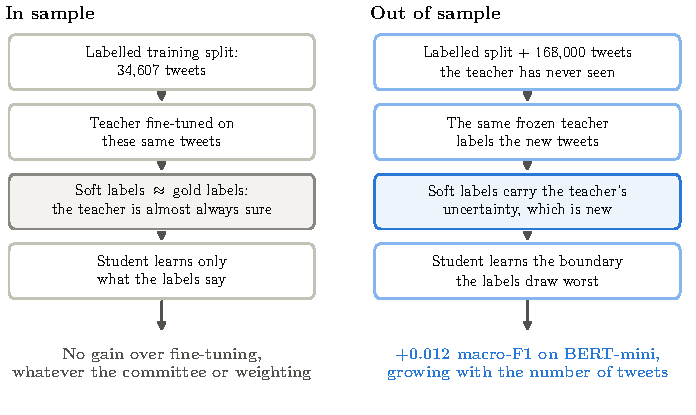
\includegraphics[width=\textwidth]{figures/fig_schematic.pdf}
\caption{In-sample against out-of-sample distillation. The same teacher and student are used in both settings; only the text on which the student imitates the teacher differs. In sample, on the tweets the teacher was fine-tuned on, its soft labels repeat the gold labels; out of sample, on tweets it has never seen, they carry its uncertainty.}
\label{fig:schematic}
\end{figure}
\section{Notation and Committee}
\label{sec:3.1}
Let $x_i$ be a text with majority label $y_i \in \{1,\dots,C\}$. A committee of $K$ teachers
produces logits $z_k(x_i) \in \mathbb{R}^C$ and masked-mean-pooled last-layer states $h_k(x_i) \in
\mathbb{R}^{d_k}$; the student produces $z_s(x_i)$ and $h_s(x_i) \in \mathbb{R}^{d_s}$, plus an
auxiliary irony head $z_s^{\text{irony}}(x_i) \in \mathbb{R}^2$. $W_k \in \mathbb{R}^{d_k \times
d_s}$ is a learned projection from the student width to teacher $k$'s width; $T$ is the distillation
temperature and $\tau$ the weight temperature.

Teachers are \emph{task-adapted}: each is initialised from a specialist checkpoint and fine-tuned on
the target training split, so that every committee member shares the task's label space. Without
this step a sarcasm model's logits are not comparable with an abuse model's and cannot enter a KL
term. The homogeneous committee $\mathcal{K}_{\text{homo}}$ is BERT-large \cite{devlin2019bert},
HateBERT \cite{caselli2021hatebert} and a Twitter irony RoBERTa \cite{barbieri2020tweeteval,
liu2019roberta}: a general encoder, a specialist in abuse that says what it means, and a specialist
in saying one thing and meaning another. The heterogeneous committee adds DeBERTa-v3-base
\cite{he2023debertav3}. The third committee adds the implicit specialist of Section~\ref{sec:3.4}.
Teachers are frozen after adaptation and their outputs cached once on every split the student will
train on; the student never sees a teacher at run time.
\section{Per-Instance Reliability}
\label{sec:3.2}
For each training instance the committee is weighted by how reliable each teacher is on it:

\begin{equation}
\ell_k(i) = \mathrm{CE}\big(\mathrm{softmax}(z_k(x_i)),\, y_i\big), \qquad
w_k(i) = \frac{\exp(-\ell_k(i)/\tau)}{\sum_{j} \exp(-\ell_j(i)/\tau)} .
\end{equation}

$w_k(i)$ is the posterior probability that teacher $k$ is the right expert for $x_i$ under a uniform
prior and a likelihood $p(y_i \mid k, x_i)^{1/\tau}$: at $\tau = 1$ it is Bayesian model averaging
over the committee on that instance; $\tau \to \infty$ recovers uniform averaging and $\tau \to 0$
hard selection of the single best teacher. Per-batch weighting, as in earlier work, replaces
$\ell_k(i)$ by its batch mean. Because the teachers are frozen and cached, $w_k(i)$ is a fixed
function of the data: it varies across instances and never across epochs or seeds, so ``dynamic''
means instance-adaptive and nothing else.
\section{Objective}
\label{sec:3.3}
\begin{equation}
\bar p(i) = \sum_k w_k(i)\, \mathrm{softmax}\!\big(z_k(x_i)/T\big), \qquad
\mathcal{L}_{\mathrm{KL}}(i) = T^2\, \mathrm{KL}\!\big(\bar p(i)\,\|\,\mathrm{softmax}(z_s(x_i)/T)\big),
\end{equation}

\begin{equation}
\mathcal{L}_{\mathrm{hid}}(i) = \sum_k w_k(i)\, \big\| W_k h_s(x_i) - h_k(x_i) \big\|_2^2, \qquad
\mathcal{L}_{\mathrm{irony}}(i) = T^2\, \mathrm{KL}\!\big(\mathrm{softmax}(z_{\text{irony}}(x_i)/T)\,\|\,\mathrm{softmax}(z_s^{\text{irony}}(x_i)/T)\big),
\end{equation}

\begin{equation}
\mathcal{L} = \frac{1}{B}\sum_i \Big[\alpha\, \mathcal{L}_{\mathrm{KL}}(i) + \beta\, m_i\, \mathrm{CE}(z_s(x_i), y_i)
 + \gamma\, \mathcal{L}_{\mathrm{hid}}(i) + \delta\, \mathcal{L}_{\mathrm{irony}}(i)\Big],
\end{equation}

with $\alpha = \beta = 0.4$, $\gamma = 0.2$, $\delta = 0.3$, $T = 4$ and $\tau = 1$ unless stated,
and $m_i \in \{0, 1\}$ a label mask that is 1 on labelled rows and 0 on the unlabelled rows of
Section~\ref{sec:3.5}. The irony teacher cannot join the committee, because its label space is irony
against non-irony, so its softened output is distilled into a second head on the student's pooled
state; the head is discarded at inference and exists to shape the shared representation. Uniform
multi-teacher distillation sets $w_k(i) = 1/K$; single-teacher distillation uses BERT-large alone;
fine-tune-only sets $\alpha = \gamma = \delta = 0$. Training: 6 epochs, AdamW
\cite{loshchilov2019decoupled} at $3 \times 10^{-5}$ ($10^{-3}$ for the BiLSTM), 10 per cent warm-up
and linear decay, batch 32, gradient clipping at 1.0, mixed precision on GPU, best validation
macro-F1 epoch kept, early stopping with patience 2, implemented in PyTorch and Transformers
\cite{paszke2019pytorch, wolf2020transformers}.
\section{The Implicit Specialist and Its Controls}
\label{sec:3.4}
No public checkpoint and neither established corpus holds knowledge of abuse by implication, so a
committee assembled from them cannot route to it. We therefore train the fourth member: HateBERT
fine-tuned on the implicit benchmark of Section~\ref{sec:4.2}, then task-adapted onto the tweet
corpus like every other teacher, its classification head re-initialised for the six-class label
space. It forms its own committee, $\mathcal{K}_{\text{spec}} = \mathcal{K}_{\text{homo}} \cup
\{\text{specialist}\}$, so that its effect is a three-seed comparison of two full committees rather
than a single ablation. Two controls accompany it, fixed before it was trained. The first distils
from the specialist alone, asking whether the committee contributes anything the specialist does
not. The second fine-tunes the same student on the implicit corpus and then on the tweet task with
no teacher, asking whether the knowledge, if any arrives, came from distillation or from the data.
\section{In Sample and Out of Sample}
\label{sec:3.5}
Every objective above is evaluated in two settings that differ only in where the teacher's function
is sampled. \emph{In sample}, the student is trained on the labelled split $\mathcal{D}$, the
teachers' outputs are cached on $\mathcal{D}$, and $\mathcal{D}$ is the split the teachers were
fine-tuned on. \emph{Out of sample}, an unlabelled transfer set $\mathcal{U}$ of texts outside every
teacher's training split is appended to $\mathcal{D}$; on $x_u \in \mathcal{U}$ the label mask $m_u
= 0$ removes the hard-label term, and the student trains from $\alpha\, \mathcal{L}_{\mathrm{KL}}(u)
+ \gamma\, \mathcal{L}_{\mathrm{hid}}(u) + \delta\, \mathcal{L}_{\mathrm{irony}}(u)$ alone. Nothing
else changes: the same objective, teachers, student, epochs and learning rate. The construction of
$\mathcal{U}$ is in Section~\ref{sec:4.4}; it is shuffled once with a fixed seed so that its
prefixes are nested subsets, which is what lets Section~\ref{sec:5.8} vary its size with everything
else fixed.

Two controls separate what the soft labels carry from what more text and more updates carry. The
\emph{hard-label} control replaces $\bar p(u)$ by the committee's $\arg\max$ and trains the transfer
rows with cross-entropy alone. The \emph{matched-steps} controls fine-tune the student with no
teacher for as many updates as a transfer arm takes (13 epochs for the 42,013-row set, 35 for the
168,000-row set), early stopping off and the best validation epoch kept, so that optimisation length
is held equal rather than argued away.

Out of sample, the reliability of Section~\ref{sec:3.2} has no label to be scored against, so we
also test a reliability the teachers cannot have memorised. Let $\mathcal{V}$ be the validation
split, $c_k(v) \in \{0, 1\}$ whether teacher $k$ is correct on $v \in \mathcal{V}$, and $N_k(x)$ the
$m$ validation texts nearest $x$ by cosine similarity in teacher $k$'s own pooled space. Then

\begin{equation}
r_k(x) = \frac{1 + \sum_{v \in N_k(x)} c_k(v)}{m + 2}, \qquad
w_k(x) = \frac{r_k(x)^{1/\tau}}{\sum_j r_j(x)^{1/\tau}},
\end{equation}

with $m = 20$ and $\tau = 1$: the weight is proportional to the teacher's local out-of-sample
accuracy, defined on labelled and unlabelled rows alike. It is a control, not a proposal:
Section~\ref{sec:5.4} sets its ceiling before any student trains on it.
\section{What Is Measured About the Weighting}
\label{sec:3.6}
A committee of specialists is only a committee if the weights go somewhere. For each teacher we
report the \emph{routing contrast}: its mean weight on instances of the class that holds indirect
abuse minus its mean weight on the classes that name their target, with a percentile bootstrap
interval over 2,000 resamples, measured in the committee the students actually trained with. With
tens of thousands of training instances almost any contrast excludes zero, so its size is read
against the uniform weight $1/K$. And because the weights are a fixed function of the data, the
sweep over $\tau$ reaches 0.05, where they are as sharp as the reliability signal allows.

\section{Training Procedure}
\label{sec:3.7}
Algorithm~\ref{alg:training} gives the procedure shared by every run. In-sample runs use an empty
transfer set; fine-tune-only runs skip the teachers and train on the labelled split with cross-entropy
alone.

\begin{algorithm}[htbp]
\caption{Distillation in and out of sample.}
\label{alg:training}
\begin{algorithmic}[1]
\Require labelled split $\mathcal{D}$; unlabelled transfer set $\mathcal{U}$, empty in sample; teacher
  checkpoints $M_1, \dots, M_K$; irony teacher $M_{\mathrm{irony}}$; pre-trained student $S$
\For{$k = 1, \dots, K$}
  \State fine-tune $M_k$ on $\mathcal{D}$, keep its best validation epoch, and freeze it \Comment{task adaptation}
\EndFor
\For{each text $x \in \mathcal{D} \cup \mathcal{U}$}
  \State cache $z_k(x)$ and $h_k(x)$ for every teacher $k$, and $z_{\mathrm{irony}}(x)$
\EndFor
\State set the label mask $m_x = 1$ for $x \in \mathcal{D}$ and $m_x = 0$ for $x \in \mathcal{U}$
\For{epoch $= 1, \dots, E$}
  \For{each minibatch $B$ drawn from $\mathcal{D} \cup \mathcal{U}$}
    \State compute $z_s(x)$, $h_s(x)$ and $z^{\mathrm{irony}}_s(x)$ for $x \in B$
    \State compute the weights $w_k(x)$ of Section~\ref{sec:3.2}, or of Section~\ref{sec:3.5} out of sample
    \State compute the loss of Section~\ref{sec:3.3} with the mask $m_x$ and update $S$ and $W_1, \dots, W_K$
  \EndFor
  \State evaluate macro-F1 on the validation split and keep the best epoch
\EndFor
\State \Return $S$, discarding the projections $W_k$ and the irony head
\end{algorithmic}
\end{algorithm}

\chapter{Datasets and Experimental Setup}
\label{ch:4}
Table~\ref{tab:data} summarises the data. The primary benchmark is a cleaned fine-grained
cyberbullying tweet corpus. A benchmark that labels implication, built from a single corpus, and
inference-only probe sets measure what the tweet corpus cannot. An unlabelled transfer set, screened
against all of them, supplies the out-of-sample text.

\begin{table}[htbp]
\centering
\small
\caption{The data used in this thesis.}
\label{tab:data}
\begin{tabular}{p{4.6cm}p{3.1cm}rrrp{1.7cm}}
\toprule
Set & Role & Train & Validation & Test & Labels \\
\midrule
Cyberbullying tweets, cleaned & primary benchmark & 34,607 & 4,326 & 4,326 & 6 classes \\
Implicit Hate Corpus, single source & implicit benchmark & 16,509 & 2,064 & 2,064 & 3 classes \\
ISHate, held out whole & out-of-domain test & -- & -- & 27,096 & 3 classes \\
Benign sarcasm probe & inference only & -- & -- & 883 & -- \\
Ironic abuse probe & inference only & -- & -- & 1,560 & -- \\
Implicit abuse probe, a subset of it & inference only & -- & -- & 763 & -- \\
Transfer set, abuse-domain base & training, unlabelled & 42,013 & -- & -- & none \\
Transfer set, extended & training, unlabelled & 205,593 & -- & -- & none \\
\bottomrule
\end{tabular}
\end{table}

\section{The Tweet Corpus}
\label{sec:4.1}
The fine-grained cyberbullying corpus \cite{wang2020sosnet} contains 47,692 tweets in six classes:
age, ethnicity, gender, religion, other\_cyberbullying and not\_cyberbullying. Repeated tweets are
common and some repeats carry different labels. We drop tweets shorter than two tokens (758), every
tweet whose normalised text appears with more than one label, all copies included (1,563 texts,
3,168 rows), and exact duplicates (507), then split the 43,259 survivors 80/10/10 stratified by
class with seed 42, asserting the splits disjoint on normalised text: 34,607 / 4,326 / 4,326. The
two classes that lose the most rows, other\_cyberbullying and not\_cyberbullying, are the two the
literature reports as confusable. A validation-to-test accuracy gap of 0.94 against 0.86 observed on
the raw corpus disappears on the cleaned split.

Table~\ref{tab:classes} gives the class distribution of the cleaned splits.

\begin{table}[htbp]
\centering
\small
\caption{Class distribution of the cleaned tweet corpus.}
\label{tab:classes}
\begin{tabular}{lrrrr}
\toprule
Class & Train & Validation & Test & Total \\
\midrule
age & 6,348 & 793 & 793 & 7,934 \\
ethnicity & 6,270 & 784 & 784 & 7,838 \\
gender & 6,020 & 753 & 753 & 7,526 \\
religion & 6,364 & 796 & 796 & 7,956 \\
other\_cyberbullying & 4,664 & 583 & 583 & 5,830 \\
not\_cyberbullying & 4,941 & 617 & 617 & 6,175 \\
\midrule
Total & 34,607 & 4,326 & 4,326 & 43,259 \\
\bottomrule
\end{tabular}
\end{table}

\section{The Implicit Benchmark}
\label{sec:4.2}
Neither the tweet corpus nor the Wikipedia corpus labels indirectness, so a model trained on either
never sees an example annotated as implicit. Two corpora annotate the distinction: the Implicit Hate
Corpus stage-1 release, 21,480 posts in three classes (not\_hate, explicit\_hate, implicit\_hate)
\cite{elsherief2021latent}, and ISHate, 28,763 original rows after excluding its augmentations and
its ToxiGen-sourced rows \cite{ocampo2023indepth}.

\textbf{The splits come from one corpus, and the reason is measured.} In the union, 95 per cent of
implicit examples come from the Implicit Hate Corpus and 89 per cent of explicit examples from
ISHate, and a TF-IDF classifier tells the two corpora apart at 0.91 macro-F1. A model trained on the
union can therefore score well on implicit-against-explicit by recognising the source. It also does
worse where it matters: on identical Implicit Hate test rows, a classical model trained on the union
reaches 0.473 F1 on implicit hate against 0.548 for the same model trained on that corpus alone,
while its aggregate macro-F1 is higher, 0.681 against 0.562, which is exactly the artefact. We
therefore build train, validation and test from the Implicit Hate Corpus and hold ISHate out whole
as a 27,096-row out-of-domain test set. Every text occurring in any probe set
(Section~\ref{sec:4.3}) is removed first, 1,581 rows across the two corpora, so that probe metrics
stay measured on text no model has trained on. Of those, 796 come from the Implicit Hate Corpus,
leaving 20,684; the tweet pipeline then removes 10 rows shorter than two tokens, 25 rows in 12 texts
carrying conflicting labels and 12 duplicates, and the remaining 20,637 are split 80/10/10 with seed
42 into 16,509 / 2,064 / 2,064, with training classes not\_hate 10,616, implicit\_hate 5,029,
explicit\_hate 864 and 108 explicit rows in the test split. ISHate loses the other 785 probe rows,
613 rows that also occur in those splits and 269 rows in 14 conflicting-label texts, which is how
its 28,763 become the 27,096 held out.

\textbf{The label is contested.} The two corpora share 629 texts. On whether a text is hateful at
all they agree on 99.7 per cent; on whether the hate is stated or implied they agree on 48.2 per
cent, the Implicit Hate Corpus labelling essentially all of the 624 shared hateful texts implicit
and ISHate labelling 324 explicit and 300 implicit. Two expert annotation efforts placing the
boundary in materially different places bounds how sharp any result on the implicit class can be,
and is the reason the benchmark's headline metric is a threshold-free ranking
(Section~\ref{sec:4.6}) rather than a decision. The benchmark is released as a build script plus a
per-row manifest (split, label, source, SHA-1 of the normalised text), so a reader can verify a
rebuild row by row without either party redistributing text.
\section{Probes}
\label{sec:4.3}
Three inference-only sets, never used for training by any model on any corpus. They are stored as
five files, because the benign-sarcasm probe keeps its unscreened and reviewed versions beside the
screened one the metrics use, and all five are screened against the transfer set. \emph{Benign
sarcasm}: 1,064 sarcastic tweets from iSarcasmEval \cite{abufarha2022semeval, oprea2020isarcasm},
author-labelled, of which 883 survive a screening pass over the rows a classical classifier flags as
abusive; the metric is the false-positive rate, the share whose argmax is any abusive class. Where a
score rather than a decision is needed, $p(\text{abusive})$ is one minus the probability of the
not-abusive class: one minus the probability of \texttt{not\_cyberbullying} on the tweet corpus, and
one minus the probability of \texttt{not\_hate} on the implicit benchmark. \emph{Ironic abuse}:
1,560 items, 797 posts labelled irony in the Implicit Hate Corpus stage-2 data and 763 original
ISHate rows labelled implicit; the metric is recall. \emph{Implicit abuse}: the 763 ISHate rows
alone. ISHate rows sourced from ToxiGen or the Implicit Hate Corpus are excluded from the probes so
that they stay independent of the corpus they test transfer into. The probes are rule-built from
published corpora, not hand-verified; a 300-item human annotation with inter-annotator agreement
\cite{fleiss1971measuring} is in progress. Probe metrics are only meaningful for models trained on
Twitter-domain data.
\section{The Transfer Set}
\label{sec:4.4}
The transfer set is unlabelled tweets the teachers have never fitted. Its base is abuse-domain text
from public corpora used as text only, their labels discarded before anything reads them: OLID
\cite{zampieri2019olid} and HatEval \cite{basile2019hateval} through TweetEval
\cite{barbieri2020tweeteval} (14,100 and 12,970 tweets), Davidson et al.
\cite{davidson2017automated} (24,783), and the 1,563 tweets of the cyberbullying corpus that our own
cleaning dropped for carrying more than one label. TweetEval's irony configuration is not used,
because it is the irony teacher's own fine-tuning data, and Founta et al. \cite{founta2018large} is
excluded under the provenance rule of Section~\ref{sec:4.5}. Every text is matched on the splits'
own normalised key against the train, validation and test splits, all five probe files and every
file of the implicit benchmark including the held-out ISHate set, and dropped on any hit; duplicates
within the set are dropped too. Of 53,416 texts, 318 are shorter than two tokens, 877 are
duplicates, 117 occur in a tweet split, 103 in the ironic- and implicit-abuse probes, 2 in the
implicit benchmark's test split and 9,988 in the held-out ISHate set, which incorporates HatEval's
tweets: \textbf{42,013 remain} (Davidson 24,139; OLID 13,760; HatEval 2,556; conflicting-label
tweets 1,558), 1.2 times the training split. The screen against ISHate matters: without it, a fifth
of the ``unlabelled'' set would have been text a later evaluation scores.

For the size curve the base set is extended with generic tweets from TweetEval's sentiment, emoji
and emotion configurations (59,899, 100,000 and 5,052 rows), screened identically and against the
base set itself: 163,580 survive (emoji 98,867, sentiment 59,715, emotion 4,998), giving 205,593
rows in all. The generic block is shuffled with the same seed before it is appended, so its sources
are mixed throughout rather than ordered by corpus. The base rows come first and verbatim, so a
prefix of the extended file up to 42,013 is the base set, prefixes below that are nested subsets of
it, and rows beyond it are generic. The size curve of Section~\ref{sec:5.8} uses the prefixes of
5,000, 10,000, 21,000, 42,013, 84,000 and 168,000 rows; the remaining 37,593 screened rows were
built and not used. Its composition control is the slice of the same file that follows the base set,
rows 42,013 to 84,026, which is 42,013 generic tweets and no abuse-domain text. The report of every
count (\texttt{transfer\_report.json}, \texttt{transfer\_big\_report.json}) is regenerated by the
run itself, with the same seed, from the same public sources; Appendix~\ref{app:transfer} says what
each file records.

Table~\ref{tab:transfer} records every count.

\begin{table}[htbp]
\centering
\small
\caption{Construction of the transfer set. Upper part: rows read and kept per source. Lower part: rows
matching each screen; a row can match more than one screen, so the screens do not sum to the difference.}
\label{tab:transfer}
\begin{tabular}{lrr}
\toprule
Source & Rows read & Rows kept \\
\midrule
\multicolumn{3}{l}{\emph{Abuse-domain base set}} \\
OLID \cite{zampieri2019olid} & 14,100 & 13,760 \\
HatEval \cite{basile2019hateval} & 12,970 & 2,556 \\
Davidson et al. \cite{davidson2017automated} & 24,783 & 24,139 \\
Conflicting-label tweets of the corpus & 1,563 & 1,558 \\
Total & 53,416 & 42,013 \\
\midrule
\multicolumn{3}{l}{\emph{Generic extension}} \\
TweetEval sentiment & 59,899 & 59,715 \\
TweetEval emoji & 100,000 & 98,867 \\
TweetEval emotion & 5,052 & 4,998 \\
Total & 164,951 & 163,580 \\
\midrule
Extended set, base first & & 205,593 \\
\midrule
Screen & Base & Extension \\
\midrule
Shorter than two tokens & 318 & 114 \\
Duplicate within the set & 877 & 1,226 \\
Occurs in a tweet split & 117 & 14 \\
Occurs in a probe set & 103 & 0 \\
Occurs in the implicit benchmark's splits & 2 & 0 \\
Occurs in held-out ISHate & 9,988 & 9 \\
Occurs in the base set & -- & 8 \\
\bottomrule
\end{tabular}
\end{table}

\section{Teachers, Students, Floor}
\label{sec:4.5}
Teachers: BERT-large-uncased (335M), HateBERT (110M), Twitter-RoBERTa-base-irony (125M),
DeBERTa-v3-base (184M), and the implicit specialist (HateBERT, 110M), each fine-tuned on the tweet
training split for 5 epochs at $2 \times 10^{-5}$, batch 32, best validation epoch kept, trained
once. A provenance rule excludes from every test set, probe and transfer set any data a teacher's
checkpoint was trained on before adaptation. Students: BERT-mini (11.2M, the headline student),
BERT-small (28.8M) \cite{turc2019wellread}, DistilBERT (67.0M) \cite{sanh2019distilbert},
DeBERTa-v3-xsmall (70.8M) \cite{he2023debertav3}, and a two-layer BiLSTM over a WordPiece vocabulary
(10.4M) \cite{tang2019distilling}; the last two are the heterogeneous students. The classical floor
is TF-IDF over word 1-2 grams and character 3-5 grams with class-balanced logistic regression:
0.8798 macro-F1 on tweets, 0.5620 on the implicit benchmark (implicit\_hate F1 0.5562,
implicit-discrimination AUC 0.7610). Every neural result is read against it.
\section{Metrics}
\label{sec:4.6}
Recall on ironic abuse at a fixed threshold cannot distinguish a model that fails to see indirect
abuse from one that sees it and cannot separate it from harmless sarcasm. We report
\textbf{sarcasm-discrimination AUC}: the ROC-AUC of $p(\text{abusive})$ with the ironic-abuse probe
as positives and the benign-sarcasm probe as negatives, threshold-free and defined identically on
every corpus, with the recall-against-false-positive curve beside it because a deployment must
choose a threshold even though an evaluation should not. On the implicit benchmark the analogue is
\textbf{implicit-discrimination AUC}, implicit-hate rows against benign rows ranked by
$p(\text{implicit hate})$; macro-F1 there is dominated by an explicit class of 108 test rows and is
reported but not argued on. Elsewhere: macro-F1, accuracy, expected calibration error
\cite{guo2017calibration}, and per-class F1.
\section{Protocol and Statistics}
\label{sec:4.7}
Three seeds per main configuration, one for ablations, controls and sweeps. Every difference the
paper states is a paired bootstrap over the test set \cite{koehn2004statistical,
dror2018hitchhiker}: seeds paired by index, 1,000 resamples per seed, the 95 per cent interval of
the pooled differences. The grid makes 99 such comparisons and they are generated as a table, not
transcribed; nine intervals exclude zero, one for removing pre-training and eight for out-of-sample
distillation. A paired interval on 4,326 posts is about 0.014 wide, so the minimum detectable
difference is about 0.007 macro-F1 \cite{card2020power}, and we say so wherever a difference is
smaller. A pre-registered stop rule required at least one task-adapted teacher to beat the
fine-tune-only student on the clean test split before any distillation ran, and the predictions for
the three out-of-sample runs were written into the decision log before each ran and scored by a
script against the tables.

\textbf{One rule constrains every table.} The same code, data and seeds produce systematically
different results on a laptop CPU and on a Kaggle T4 (Chapter~\ref{ch:7}), so every number comes
from the Kaggle grid alone. Comparisons within it are valid because everything in it was trained
identically; numbers produced elsewhere are excluded rather than reconciled. The tweet grid is
complete: 179 student runs in 18.4 GPU-hours over the five Kaggle sessions that ran to completion.
The Wikipedia grid and the student grid on the implicit benchmark are not run and are named where
they would bear on a claim.

\section{Implementation and Compute}
\label{sec:4.8}
Every student and teacher in this thesis was trained on Kaggle T4 accelerators by one driver script that
resumes finished work from the previous session's output, so that the grid could grow across sessions
of at most twelve hours. Table~\ref{tab:sessions} lists the sessions of the tweet notebook. Two sessions
failed and are reported rather than hidden: the second stopped at teacher caching because the resume
logic had discarded the teacher weights, and the third froze inside a diagnostic cell until Kaggle ended
it; both faults were fixed, and the driver now kills any command that writes nothing for two hours. The
teachers, the implicit specialist and the student pre-trained on the implicit corpus were each trained
once and resumed by every later session. The code, the driver, the notebook and a CPU smoke test that runs
every stage on tiny models before any GPU session are in the repository.

\begin{table}[htbp]
\centering
\small
\caption{The Kaggle sessions of the tweet grid.}
\label{tab:sessions}
\begin{tabular}{clrr}
\toprule
Session & What it added & GPU-hours & Student runs, cumulative \\
\midrule
1 & the in-sample grid on five students and three committees & 8.24 & 120 \\
2 & failed at teacher caching; fixed & -- & 120 \\
3 & froze in a diagnostic cell; fixed & -- & 120 \\
4 & specialist committee, controls, sharpest temperatures & 1.41 & 131 \\
5 & the five out-of-sample arms & 2.11 & 146 \\
6 & the size curve and its first controls & 3.52 & 170 \\
7 & the 35-epoch control and two more students & 3.16 & 179 \\
\midrule
 & total of the completed sessions & 18.44 & 179 \\
\bottomrule
\end{tabular}
\end{table}

\chapter{Results and Analysis}
\label{ch:5}
The sections run in the order of the argument, not the order the runs were made: the in-sample audit
(5.1 to 5.5), its mechanism (5.6), the out-of-sample result and its curve (5.7 and 5.8), what never
transferred (5.9), what survives for practice (5.10), and the decision each research question comes
to on this evidence (5.11). Every difference is a paired bootstrap interval; single-seed rows are
marked and treated as indicative.
\section{The Teachers Clear the Bar}
\label{sec:5.1}
\begin{table}[htbp]
\centering
\small
\caption[Teachers after task adaptation]{Teachers after task adaptation, with the classical floor. The training loss is the last epoch's cross-entropy on the split the students are distilled on; the probe columns are the share of each probe the model assigns to any abusive class, which is its argmax decision rather than a threshold on $p(\text{abusive})$.}
\label{tab:teachers}
\begin{adjustbox}{max width=\textwidth}
\begin{tabular}{lcccccc}
\toprule
Teacher & Macro-F1 & Accuracy & ECE & Training loss, last epoch & Benign-sarcasm FPR & Ironic-abuse recall \\
\midrule
BERT-large & 0.8973 & 0.9075 & 0.056 & 0.033 & 0.224 & 0.585 \\
Implicit specialist, task-adapted & 0.8931 & 0.9043 & 0.072 & 0.061 & 0.263 & 0.678 \\
RoBERTa-irony, task-adapted & 0.8926 & 0.9050 & 0.067 & 0.077 & 0.294 & 0.718 \\
HateBERT, task-adapted & 0.8887 & 0.9011 & 0.076 & 0.059 & 0.317 & 0.696 \\
DeBERTa-v3-base & 0.8720 & 0.8867 & 0.053 & 0.227 & 0.409 & 0.773 \\
TF-IDF + logistic regression & 0.8798 & 0.8930 & -- & -- & -- & -- \\
\bottomrule
\end{tabular}
\end{adjustbox}
\end{table}

Table~\ref{tab:teachers} reports the teachers after task adaptation. Three of the original four beat
the fine-tune-only headline student and the classical floor, so the pre-registered stop rule passes.
DeBERTa-v3-base sits below the floor and is retained only as the heterogeneous committee member,
which is what it is there to test. The implicit specialist, trained on different data under a
different label scheme, lands within 0.005 of the other three after adaptation. Two columns of this
table carry the rest of the paper. The training losses say that every task-adapted teacher has, by
its last epoch, assigned the gold label a probability near one on the split the student will be
distilled on (Section~\ref{sec:5.6}). And the probe columns already show the pattern
Section~\ref{sec:5.9} makes precise: ordered by false-positive rate on harmless sarcasm, the
teachers are almost exactly ordered by recall on ironic abuse.
\section{In Sample, Distillation Raises Every Student by Less Than the Test Set Can Resolve}
\label{sec:5.2}
Table~\ref{tab:main} gives the in-sample grid: test macro-F1 of every student under every objective
and committee, against a classical floor of 0.8798.

\begin{table}[htbp]
\centering
\small
\caption[In-sample distillation on the five students]{In-sample distillation: test macro-F1 of the five students under each objective and committee, mean over three seeds. The classical floor is 0.8798. Standard deviations over seeds run from 0.0002 to 0.0078 and are in the generated table \texttt{paper/tables/main.csv}; the paired intervals are in Appendix~\ref{app:significance}.}
\label{tab:main}
\begin{adjustbox}{max width=\textwidth}
\begin{tabular}{lccccccc}
\toprule
Student & Params & Fine-tune only & Single-teacher & Uniform & D-MTHD & Uniform + DeBERTa & D-MTHD + DeBERTa \\
\midrule
BERT-mini & 11.2M & 0.8393 & 0.8405 & 0.8385 & 0.8378 & 0.8378 & 0.8373 \\
BERT-small & 28.8M & 0.8469 & 0.8488 & 0.8505 & 0.8471 & 0.8509 & 0.8477 \\
DistilBERT & 67.0M & 0.8907 & 0.8963 & 0.8960 & 0.8960 & 0.8975 & 0.8966 \\
DeBERTa-v3-xsmall & 70.8M & 0.8825 & 0.8865 & 0.8862 & 0.8833 & 0.8847 & 0.8828 \\
BiLSTM & 10.4M & 0.8693 & 0.8748 & 0.8761 & 0.8732 & 0.8760 & 0.8764 \\
\bottomrule
\end{tabular}
\end{adjustbox}
\end{table}

Best distilled configuration against fine-tune-only: BERT-mini +0.0012 [$-$0.0057, +0.0079],
BERT-small +0.0040 [$-$0.0058, +0.0126], DistilBERT +0.0068 [$-$0.0013, +0.0139], DeBERTa-v3-xsmall
+0.0040 [$-$0.0024, +0.0109], BiLSTM +0.0071 [$-$0.0039, +0.0195]. Five of five positive, which is
the result the control was added to test; and none of the five intervals excludes zero, nor does any
of the 27 in-sample distillation-against-fine-tuning comparisons in the grid. Taking the best of six
configurations per student also flatters the difference. The supportable claim is the modest one: in
sample, distillation moves every student in the same direction, by 0.001 to 0.007 macro-F1, which a
test set of 4,326 posts cannot resolve.

Two students deserve a remark. The most heterogeneous student, the BiLSTM, gains the most, and the
student that shares the teachers' architecture most closely, BERT-mini, gains the least; the
hidden-state term, the only part of the objective that architectural similarity could help, is worth
+0.0009 on BERT-mini. Nothing in this grid supports a preference for homogeneous student and
teachers. And on BERT-mini no distilled configuration beats the no-teacher control by more than the
seeds' own spread: candidate minus fine-tune-only is $-$0.0015 [$-$0.0076, +0.0048] for D-MTHD,
$-$0.0007 [$-$0.0074, +0.0058] for uniform, +0.0012 [$-$0.0057, +0.0079] for single-teacher,
$-$0.0019 [$-$0.0082, +0.0041] with the DeBERTa committee, $-$0.0003 [$-$0.0080, +0.0075] and
$-$0.0019 [$-$0.0093, +0.0049] with the specialist committee under averaging and weighting.

The efficiency claim sits in this table. DistilBERT with a uniform heterogeneous committee reaches
0.8975 against BERT-large's 0.8973 at a fifth of the parameters and latency
(Section~\ref{sec:5.10}). We state that as parity, not as the student beating the teacher.
\section{Per-Instance Weighting Does Not Differ from Uniform Averaging at Any Temperature}
\label{sec:5.3}
\begin{table}[htbp]
\centering
\small
\caption[Per-instance weighting minus uniform averaging]{Per-instance weighting minus uniform averaging, with and without the DeBERTa teacher; paired bootstrap 95\% intervals.}
\label{tab:dmthd-uniform}
\begin{adjustbox}{max width=\textwidth}
\begin{tabular}{lcc}
\toprule
Student & D-MTHD minus uniform & Same, with DeBERTa \\
\midrule
BERT-mini & $-$0.0007 [$-$0.0074, +0.0061] & $-$0.0005 [$-$0.0067, +0.0054] \\
BERT-small & $-$0.0034 [$-$0.0106, +0.0036] & $-$0.0032 [$-$0.0100, +0.0033] \\
DistilBERT & +0.0000 [$-$0.0079, +0.0082] & $-$0.0010 [$-$0.0087, +0.0069] \\
DeBERTa-v3-xsmall & $-$0.0029 [$-$0.0086, +0.0029] & $-$0.0019 [$-$0.0108, +0.0108] \\
BiLSTM & $-$0.0029 [$-$0.0116, +0.0056] & +0.0004 [$-$0.0072, +0.0081] \\
\bottomrule
\end{tabular}
\end{adjustbox}
\end{table}

Table~\ref{tab:dmthd-uniform} sets the weighting against averaging on every student. Without the
DeBERTa teacher four differences are negative and one is a tie; with it, four are negative and one
positive. Every interval contains zero. On the headline student the ablation that removes the
weighting altogether scores 0.8386 against 0.8385 for full D-MTHD on the same seed.

The obvious objection is that at $\tau = 1$ the weights are nearly uniform, 0.332 / 0.337 / 0.331
against 0.333, so the two objectives coincide by arithmetic. The sweep therefore reaches $\tau =
0.05$ (Table~\ref{tab:tau}, Figure~\ref{fig:tau}).

\begin{table}[htbp]
\centering
\small
\caption[Teacher weights and score across the temperature sweep]{The weighting-temperature sweep on BERT-mini: mean weight of each teacher over the training split, and test macro-F1 of the first seed.}
\label{tab:tau}
\begin{adjustbox}{max width=\textwidth}
\begin{tabular}{lcc}
\toprule
$\tau$ & Mean weights, BERT-large / HateBERT / irony & Test macro-F1, seed 1 \\
\midrule
0.05 & 0.318 / 0.356 / 0.326 & 0.8392 \\
0.1 & 0.323 / 0.349 / 0.328 & 0.8388 \\
0.2 & 0.327 / 0.344 / 0.329 & 0.8385 \\
0.5 & 0.330 / 0.340 / 0.330 & 0.8390 \\
1 (default) & 0.332 / 0.337 / 0.331 & 0.8385 \\
2 & 0.332 / 0.336 / 0.332 & 0.8390 \\
5 & 0.333 / 0.334 / 0.333 & 0.8389 \\
Uniform averaging & 0.333 each & 0.8372 \\
Fine-tune only & -- & 0.8394 \\
\bottomrule
\end{tabular}
\end{adjustbox}
\end{table}

\begin{figure}[htbp]
\centering
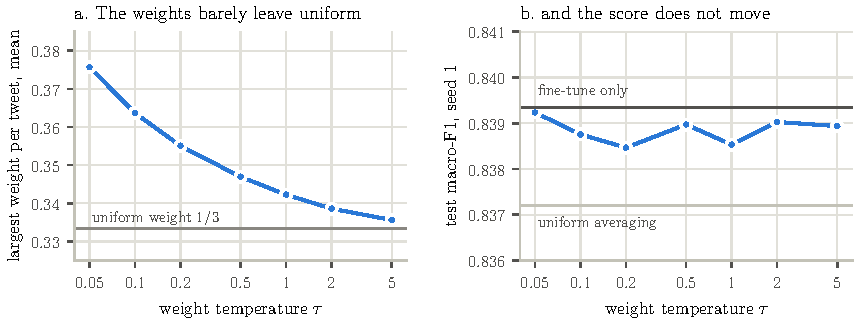
\includegraphics[width=\textwidth]{figures/fig_tau.pdf}
\caption[The weighting-temperature sweep on BERT-mini]{The weighting-temperature sweep on BERT-mini. (a) Even at $\tau = 0.05$ the largest teacher weight on a tweet averages 0.376 against a uniform 0.333. (b) Test macro-F1 of the first seed stays within 0.0007 across a hundredfold range of $\tau$, below fine-tuning at every value.}
\label{fig:tau}
\end{figure}

Across a hundredfold range of temperature the score stays inside 0.0007 and below fine-tune-only at
every value; the sharpest setting differs from the default by +0.0007 [$-$0.0008, +0.0023] and from
uniform averaging by +0.0020 [$-$0.0042, +0.0077]. The weights barely sharpen: even at $\tau = 0.05$
the heaviest teacher averages 0.356.

\textbf{Ablations and sweeps say the same.} BERT-mini, one seed, against full D-MTHD at 0.8378:
randomly initialised student 0.7905 ($-$0.0473); no auxiliary irony head 0.8364 ($-$0.0014); no
hidden-state term 0.8369 ($-$0.0009); uniform weights 0.8386 (+0.0008); per-batch weights 0.8389
(+0.0011); the specialist alone 0.8392 (+0.0014); pre-trained on the implicit corpus 0.8377
($-$0.0001). Removing components of the method costs at most 0.0014 and in three cases improves the
score; removing pre-training costs 0.047, and against fine-tune-only on the same seed it is the one
in-sample difference in the grid whose interval excludes zero, $-$0.0488 [$-$0.0603, $-$0.0376].
Hyper-parameters behave the same way, against 0.8385 at the defaults on the same seed: $T \in \{1,
2, 8\}$ gives 0.8386 / 0.8402 / 0.8391, $\alpha \in \{0.2, 0.6\}$ 0.8386 / 0.8394, $\delta \in
\{0.1, 0.5\}$ 0.8389 / 0.8399. The objective is flat in every direction we can move it, and adding a
DeBERTa-v3 teacher to the homogeneous committee changes the five students by $-$0.0005, +0.0006,
+0.0032, $-$0.0005 and +0.0006.
\section{The Committee Is Worth More Than Its Best Member, and the Student Receives None of It}
\label{sec:5.4}
Table~\ref{tab:committee} scores the teachers' saved test probabilities directly, before any student
is involved.

\begin{table}[htbp]
\centering
\small
\caption[Combining the teachers directly on the test set]{Combining the teachers directly on the test set, before any student is trained: macro-F1 of each combination rule and the oracle's accuracy.}
\label{tab:committee}
\begin{adjustbox}{max width=\textwidth}
\begin{tabular}{lccccccc}
\toprule
Committee & Best single & Uniform mean & Confidence-weighted & Entropy-weighted & Most confident teacher & Stacked gate (5-fold CV) & Oracle accuracy \\
\midrule
Homogeneous (3) & 0.8973 & 0.9026 & 0.9018 & 0.9023 & 0.9015 & 0.9046 & 0.9454 \\
+ implicit specialist (4) & 0.8973 & 0.9000 & 0.9005 & 0.9011 & 0.9011 & 0.9043 & 0.9494 \\
+ DeBERTa (4) & 0.8973 & 0.9051 & 0.9055 & 0.9052 & 0.9005 & 0.9055 & 0.9526 \\
All five & 0.8973 & 0.9036 & 0.9046 & 0.9030 & 0.9000 & 0.9041 & 0.9552 \\
\bottomrule
\end{tabular}
\end{adjustbox}
\end{table}

Uniform averaging of the committee beats the best teacher by 0.3 to 0.8 macro-F1. No combination
that needs no gold label at inference improves on the uniform mean by more than 0.005, and neither
does a stacked logistic-regression gate fitted to the concatenated teacher probabilities by
five-fold cross-validation over the test set, which is as favourable a test of learned routing as
can be made without touching the training data. The oracle that picks a correct teacher whenever one
exists sits at 0.945 to 0.955 accuracy, against 0.9075 for BERT-large. That headroom is real and it
is unreachable from the teachers' outputs: where the teachers disagree, 10 to 14 per cent of the
test set, some teacher is right on about 90 per cent of items and the uniform mean on 55 to 62, and
their probabilities do not say which. A corrected reliability signal therefore has a ceiling of
under half a point of macro-F1 over uniform averaging on this committee, in or out of sample.

The teachers are not diverse enough for a weighting to have work to do, and adaptation is what made
them so (Table~\ref{tab:agreement}, Figure~\ref{fig:agreement}).

\begin{table}[htbp]
\centering
\small
\caption{Agreement between the task-adapted teachers on the test set.}
\label{tab:agreement}
\begin{adjustbox}{max width=\textwidth}
\begin{tabular}{lccc}
\toprule
Teacher pair & Cohen's kappa & Disagreement & Error overlap \\
\midrule
BERT-large, HateBERT & 0.920 & 6.7\% & 0.710 \\
BERT-large, irony & 0.922 & 6.4\% & 0.712 \\
BERT-large, DeBERTa-v3 & 0.893 & 8.9\% & 0.712 \\
HateBERT, irony & 0.916 & 7.0\% & 0.673 \\
HateBERT, DeBERTa-v3 & 0.889 & 9.2\% & 0.673 \\
irony, DeBERTa-v3 & 0.900 & 8.3\% & 0.730 \\
BERT-large, implicit specialist & 0.924 & 6.4\% & 0.710 \\
\textbf{HateBERT, implicit specialist} & \textbf{0.962} & \textbf{3.1\%} & \textbf{0.843} \\
irony, implicit specialist & 0.918 & 6.8\% & 0.689 \\
implicit specialist, DeBERTa-v3 & 0.889 & 9.2\% & 0.691 \\
\bottomrule
\end{tabular}
\end{adjustbox}
\end{table}

\begin{figure}[htbp]
\centering
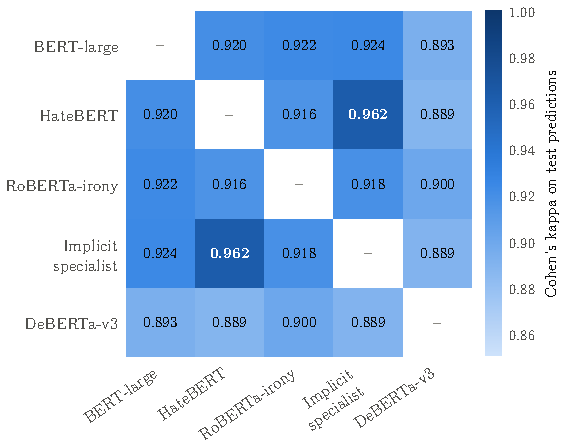
\includegraphics[width=\textwidth]{figures/fig_agreement.pdf}
\caption[Pairwise agreement between the task-adapted teachers]{Cohen's kappa between the task-adapted teachers' test predictions. Every pair agrees above 0.88, and the implicit specialist agrees with HateBERT, the checkpoint it was trained from, at 0.962. A per-instance weighting has to work inside what is left.}
\label{fig:agreement}
\end{figure}

The original four teachers are all right on 83.2 per cent of the test set and all wrong on the same
4.7 per cent. A per-instance weighting can only express a preference where its members disagree, at
most one instance in seven here, and on about half of the best teacher's errors no member is right
to prefer. The committee was chosen for complementary expertise, and after task adaptation on the
same corpus its members converged to near-identical behaviour. Task adaptation is what makes a
sarcasm model's logits comparable with an abuse model's, and it is also what removes the diversity
the combination was meant to exploit. \textbf{Task adaptation buys comparability and spends
diversity}, and any cross-task committee faces the trade.

The students do not receive even the 0.3 to 0.8 that the committee has. Uniform multi-teacher
against single-teacher distillation is $-$0.0019 [$-$0.0077, +0.0038], +0.0017 [$-$0.0070, +0.0115],
$-$0.0003 [$-$0.0070, +0.0060], $-$0.0003 [$-$0.0072, +0.0070] and +0.0014 [$-$0.0073, +0.0099]
across the five students. A better label on the same 34,607 training texts does not make a better
student, and Section~\ref{sec:5.6} says why: on those texts the label is not better.
\section{A Teacher That Has Seen Implication Labelled Does Not Help Either}
\label{sec:5.5}
The implicit specialist is the sharpest case of the previous section. It learned from a different
corpus under a different label scheme, and it comes back from adaptation as the closest thing in the
committee to HateBERT, the model it started from: kappa 0.962, disagreement on 3.1 per cent of the
test set, 84 per cent of HateBERT's errors made by the specialist as well. It raises the oracle over
the committee only from 0.9526 to 0.9552. Table~\ref{tab:specialist} gives the specialist and its
two controls on the headline student.

\begin{table}[htbp]
\centering
\small
\caption{The implicit specialist and its controls on BERT-mini.}
\label{tab:specialist}
\begin{adjustbox}{max width=\textwidth}
\begin{tabular}{lcccc}
\toprule
Configuration & Seeds & Macro-F1 & F1 on other\_cyberbullying & Sarcasm-discrimination AUC (seed 1) \\
\midrule
Fine-tune only & 3 & 0.8393 $\pm$ 0.0003 & 0.707 & 0.773 \\
Uniform, homogeneous committee & 3 & 0.8385 $\pm$ 0.0018 & 0.700 & 0.774 \\
Uniform, + implicit specialist & 3 & 0.8390 $\pm$ 0.0035 & 0.699 & 0.768 \\
D-MTHD, homogeneous committee & 3 & 0.8378 $\pm$ 0.0011 & 0.705 & 0.773 \\
D-MTHD, + implicit specialist & 3 & 0.8373 $\pm$ 0.0025 & 0.697 & 0.768 \\
Specialist alone, no committee & 1 & 0.8392 & 0.709 & 0.767 \\
Pre-trained on the implicit corpus, no teacher & 1 & 0.8377 & 0.705 & 0.756 \\
\bottomrule
\end{tabular}
\end{adjustbox}
\end{table}

Adding the specialist changes macro-F1 by +0.0005 [$-$0.0059, +0.0064] under averaging and $-$0.0005
[$-$0.0069, +0.0055] under weighting; F1 on the class that holds indirect abuse and the
discrimination AUC both fall slightly. Neither control does better: the specialist alone sits within
0.0002 of the no-teacher student, and putting the implicit corpus into the student directly, by
pre-training on it, gives the lowest discrimination AUC of the in-sample models analysed.

The weights do lean towards the specialist, a little, and less than towards HateBERT. Measured in
the committee the students trained with, on the training split, as mean weight on
other\_cyberbullying minus mean weight on the four targeted classes, against a uniform weight of
0.25 (Table~\ref{tab:routing}).

\begin{table}[htbp]
\centering
\small
\caption[Routing contrast in the committee with the specialist]{Routing contrast in the committee with the specialist: mean weight on other\_cyberbullying minus mean weight on the four targeted classes, with 95\% bootstrap intervals. The uniform weight is 0.25.}
\label{tab:routing}
\begin{adjustbox}{max width=\textwidth}
\begin{tabular}{lcc}
\toprule
Teacher (committee with the specialist) & $\tau$ = 0.05 & $\tau$ = 1 \\
\midrule
HateBERT & +0.0235 [+0.0209, +0.0260] & +0.0044 [+0.0034, +0.0055] \\
Implicit specialist & +0.0187 [+0.0163, +0.0212] & +0.0027 [+0.0018, +0.0036] \\
RoBERTa-irony & $-$0.0075 [$-$0.0101, $-$0.0048] & $-$0.0011 [$-$0.0021, +0.0001] \\
BERT-large & $-$0.0347 [$-$0.0375, $-$0.0317] & $-$0.0060 [$-$0.0074, $-$0.0046] \\
\bottomrule
\end{tabular}
\end{adjustbox}
\end{table}

With tens of thousands of instances almost any contrast excludes zero, so the size is the evidence.
At the temperature the students trained with, the specialist's shift is a hundredth of the uniform
weight, and it is not specific to the specialist: HateBERT, which never saw the implicit corpus,
gains more, as the kappa predicts. And because the weights come from cross-entropy against the gold
label, a shift says only that a teacher fits other\_cyberbullying better than the targeted classes,
not that it reads implication. On this corpus, a teacher that has learned implication from labelled
data passes nothing a compact student's decisions can use, whether weighted, averaged, used alone or
replaced by pre-training on its data.
\section{Why Nothing Moved: The Soft Labels Are the Gold Labels in Sample}
\label{sec:5.6}
The weights are computed from cached teacher logits on the training split, the split each teacher
was fine-tuned on, and the student is distilled on the same split. By their last epoch the teachers'
training losses are 0.033 (BERT-large), 0.059 (HateBERT), 0.077 (irony), 0.061 (implicit specialist)
and 0.227 (DeBERTa-v3-base). On the data the weights are read from, every task-adapted teacher
assigns the gold label a probability near one on nearly every instance, cross-entropy differences
between them are a few hundredths, and the softmax of Section~\ref{sec:3.2} is flat at any
temperature that does not amplify noise. The one teacher that did not memorise the split, DeBERTa,
is the one whose weight moves (0.233 in a committee of four). The reliability signal is measuring
memorisation, not reliability, and this is a property of the error-weighted family \cite{wu2021one,
zhang2022confidence}, not of our implementation: any scheme that scores reliability against the gold
label on the training data will find every fine-tuned teacher equally reliable there.

The same fact bears on the distillation itself. On the training split the teachers' soft labels are
close to the one-hot gold labels, so the KL term carries little that the cross-entropy term does
not, and single-teacher, uniform and weighted distillation all reduce to fine-tuning with a slightly
smoothed target. This is the hazard of distilling a memorising teacher on its own training data
\cite{stanton2021does, beyer2022knowledge}, and it explains Section~\ref{sec:5.4} from the student's
side: the committee's half point exists on the test set, where the teachers are uncertain, and not
on the training set, where they are not. It also says where to look. If a teacher's soft labels
carry information only where the teacher is uncertain, the student should be distilled on text the
teacher has never fitted. The rest of the results test that sentence.
\section{Out of Sample, the Gain Appears, and It Is in the Data, Not the Committee}
\label{sec:5.7}
A transfer set of 42,013 unlabelled tweets (Section~\ref{sec:4.4}) was appended to training; on
those rows the student has no gold label and trains on the committee's soft labels and hidden states
alone. Table~\ref{tab:oos} reports five arms on BERT-mini, three seeds each, beside the in-sample
runs of the same objectives; the predictions were written before the run and are scored in
Appendix~\ref{app:predictions}.

\begin{table}[htbp]
\centering
\small
\caption[Out-of-sample distillation on BERT-mini]{Out-of-sample distillation on BERT-mini with the 42,013-tweet transfer set: the same objectives with and without the unlabelled rows, three seeds each. The labelled-split column gives each objective's in-sample twin; for the out-of-sample-weighted arm that twin is D-MTHD, because the weighting differs only where there are no labels.}
\label{tab:oos}
\begin{adjustbox}{max width=\textwidth}
\begin{tabular}{lccc}
\toprule
Objective & Labelled split only & + transfer set & Gain over fine-tune only \\
\midrule
Fine-tune only & 0.8393 $\pm$ 0.0003 & -- & -- \\
Single teacher (BERT-large) & 0.8405 $\pm$ 0.0017 & 0.8466 $\pm$ 0.0016 & +0.0073 [$-$0.0003, +0.0150] \\
Uniform committee & 0.8385 $\pm$ 0.0018 & 0.8462 $\pm$ 0.0016 & +0.0070 [$-$0.0001, +0.0144] \\
Uniform committee + DeBERTa & 0.8378 $\pm$ 0.0024 & 0.8477 $\pm$ 0.0026 & +0.0084 [+0.0007, +0.0164] \\
Out-of-sample-weighted committee (Section~\ref{sec:3.5}) & 0.8378 $\pm$ 0.0011 & 0.8484 $\pm$ 0.0011 & +0.0091 [+0.0020, +0.0165] \\
Committee's hard pseudo-labels, cross-entropy only & -- & 0.8412 $\pm$ 0.0013 & +0.0020 [$-$0.0062, +0.0104] \\
\bottomrule
\end{tabular}
\end{adjustbox}
\end{table}

The transfer set is the first intervention in the grid that moves the headline student: every one of
the twelve soft-label seeds (0.8444 to 0.8501) lies above every fine-tune-only seed (0.8389 to
0.8395), two of the four soft-label arms exclude zero, and the transfer set's own effect on the
committee is +0.0077 [+0.0000, +0.0155]. The gain is the same whatever the labeller: the four
soft-label arms lie within 0.0022 of each other, the committee is not a better labeller than one
teacher ($-$0.0003 [$-$0.0061, +0.0056]), and the out-of-sample reliability weighting adds +0.0021
[$-$0.0017, +0.0082] over averaging, inside the ceiling Section~\ref{sec:5.4} set for it; its
weights stay near uniform because the teachers' local accuracies on the transfer set differ by 0.03.
Hard pseudo-labels on the same text, with the same number of optimisation steps, gain +0.0020, so
most of the gain is carried by the soft labels (their share against hard labels, +0.0050 [$-$0.0016,
+0.0118], has an interval that includes zero). It lands where the in-sample runs never moved: F1 on
other\_cyberbullying rises from 0.707 to between 0.710 and 0.720 and on not\_cyberbullying from
0.644 to between 0.655 and 0.663, the two classes that confuse each other.

We pre-registered a threshold of 0.010 for the committee arm and it was not met; the two arms that
clear zero were not the pre-registered one, and we report the family as consistent rather than any
arm as decisive. What the run established is the direction: the gain is in the data the student
imitates on, not in the committee, its weighting or its specialist, and it is a distillation result
rather than a multi-teacher one. Two things it left open, the slope and the optimisation-length
confound, are the subject of the next section.
\section{The Gain Grows with the Transfer Set, from Any Tweets, and Survives Matched Compute}
\label{sec:5.8}
Two further runs measured the slope and the confounds, each with its predictions written before it
ran (decisions D20 and D21) and scored by a script against the tables. One teacher labels, since the
committee labelled no better; BERT-mini, three seeds per arm, six epochs as everywhere else. The
transfer set's prefixes are nested subsets; beyond its 42,013 abuse-domain tweets it is extended
with generic tweets, screened identically, to 205,593 rows. Three controls: the same number of
generic tweets as the base set, the size held fixed while the composition changes; fine-tuning alone
for 13 epochs, the 42,013-row arm's number of updates; and fine-tuning alone for 35 epochs, the
168,000-row arm's number of updates, both with early stopping off and the best validation epoch
kept.

\begin{table}[htbp]
\centering
\small
\caption[The size curve and its controls]{The size curve and its controls on BERT-mini, one teacher labelling, three seeds per arm. Gains are paired bootstrap 95\% intervals against fine-tuning.}
\label{tab:size-curve}
\begin{adjustbox}{max width=\textwidth}
\begin{tabular}{lccc}
\toprule
Arm & Transfer rows & Macro-F1 & Gain over fine-tune only \\
\midrule
Fine-tune only & 0 & 0.8393 $\pm$ 0.0003 & -- \\
Fine-tune only, 13 epochs (42k arm's updates) & 0 & 0.8420 $\pm$ 0.0021 & +0.0027 [$-$0.0040, +0.0096] \\
Fine-tune only, 35 epochs (168k arm's updates) & 0 & 0.8380 $\pm$ 0.0033 & $-$0.0013 [$-$0.0106, +0.0072] \\
42k generic tweets (composition control) & 42,013 & 0.8445 $\pm$ 0.0044 & +0.0053 [$-$0.0048, +0.0146] \\
5k abuse-domain & 5,000 & 0.8402 $\pm$ 0.0015 & +0.0010 [$-$0.0056, +0.0074] \\
10k abuse-domain & 10,000 & 0.8428 $\pm$ 0.0003 & +0.0035 [$-$0.0027, +0.0099] \\
21k abuse-domain & 21,000 & 0.8436 $\pm$ 0.0016 & +0.0043 [$-$0.0026, +0.0116] \\
42k abuse-domain & 42,013 & 0.8463 $\pm$ 0.0009 & +0.0070 [$-$0.0003, +0.0144] \\
84k: 42k abuse-domain + 42k generic & 84,000 & 0.8474 $\pm$ 0.0056 & +0.0081 [$-$0.0030, +0.0203] \\
168k: 42k abuse-domain + 126k generic & 168,000 & \textbf{0.8516 $\pm$ 0.0012} & \textbf{+0.0123 [+0.0035, +0.0211]} \\
\bottomrule
\end{tabular}
\end{adjustbox}
\end{table}

\begin{figure}[htbp]
\centering
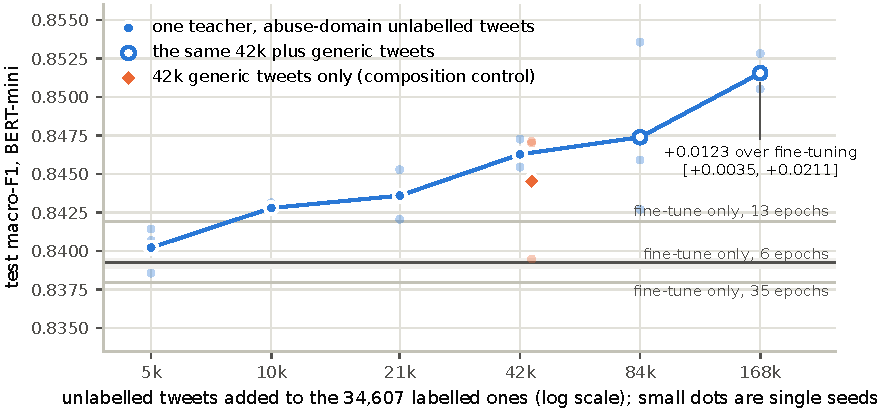
\includegraphics[width=\textwidth]{figures/fig_size_curve.pdf}
\caption[The size curve on BERT-mini]{The size curve on BERT-mini, one teacher labelling. Filled points: nested subsets of the abuse-domain transfer set; hollow points: the same set extended with generic tweets; diamond: 42,013 generic tweets alone. Horizontal lines: fine-tuning alone for 6, 13 and 35 epochs, the last two matching the number of updates of the 42k and 168k arms. Small dots are single seeds.}
\label{fig:size-curve}
\end{figure}

\textbf{The curve rises at every step} (Table~\ref{tab:size-curve}, Figure~\ref{fig:size-curve}).
Six sizes give six ordered means with no inversion, the 42k arm reproduces Section~\ref{sec:5.7}'s
to within 0.0003, and at 168k the gain is +0.0123 with an interval that excludes zero: the largest
gain in the grid on the headline student, and one of three arms that beat fine-tuning by more than
the test set can resolve. No single step of the curve is significant on its own (the largest, 84k to
168k, is +0.0042 [$-$0.0047, +0.0134]); the evidence is the ordering, and the endpoint.

\textbf{Composition matters less than we predicted.} We expected generic tweets of the same size to
gain at least 0.003 less than the abuse-domain set; they gain 0.0017 less (+0.0017 [$-$0.0066,
+0.0113]), with two of three seeds level with the abuse-domain arm. Text from the same platform
carries most of the value, which makes the recipe cheaper than we assumed: the unlabelled text need
not be abuse-related, only in the register the student will meet. Returns diminish, as predicted:
the abuse-domain rows added 1.7 points of macro-F1 per 10,000, the generic rows appended beyond them
0.4.

\textbf{Optimisation length does not explain the curve} (Figure~\ref{fig:validation}). Fine-tuning
for the 42k arm's number of updates gains +0.0027; fine-tuning for the 168k arm's number of updates
gains nothing, $-$0.0013 [$-$0.0106, +0.0072], with the validation score peaking between epochs 6
and 13 and declining afterwards (0.855 to 0.844 by the last epoch): the extra updates are spent
overfitting. The 13-epoch control's small gain was a longer search over checkpoints rather than a
better optimum, and 35 epochs is its ceiling. Against these controls the 42k arm keeps +0.0043
[$-$0.0032, +0.0122]; the 168k arm keeps +0.0096 [+0.0000, +0.0191] over the 13-epoch control and
+0.0136 [+0.0023, +0.0240], the latter with an interval clear of zero.

\begin{figure}[htbp]
\centering
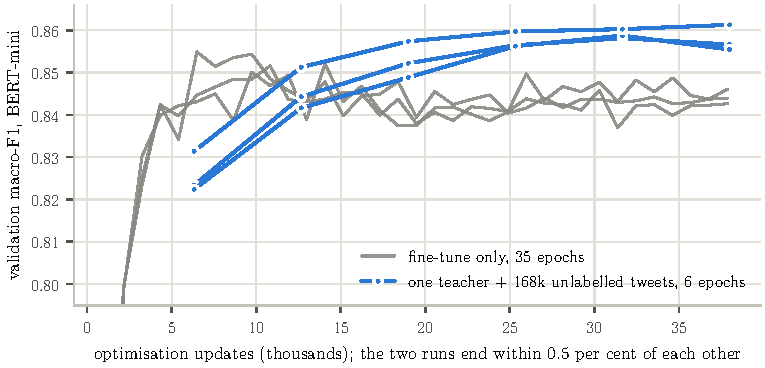
\includegraphics[width=\textwidth]{figures/fig_validation.pdf}
\caption[Validation macro-F1 against optimisation updates]{Validation macro-F1 of BERT-mini against the number of optimisation updates. Fine-tuning alone for 35 epochs (gray, three seeds) peaks early and then declines; the 168k transfer arm (blue, three seeds) reaches a higher score within the same number of updates.}
\label{fig:validation}
\end{figure}

\textbf{The endpoint holds on two more students} (Table~\ref{tab:students},
Figure~\ref{fig:students}). The largest set was run on BERT-small (28.8M, the same family) and on
the BiLSTM (10.4M, the heterogeneous student), beside their in-sample fine-tuning and single-teacher
runs:

\begin{table}[htbp]
\centering
\small
\caption{The largest transfer set on three students, three seeds each.}
\label{tab:students}
\begin{adjustbox}{max width=\textwidth}
\begin{tabular}{lccccc}
\toprule
Student & Fine-tune only & Single teacher, in sample & + 168k transfer rows & Gain over fine-tuning & Gain over the same teacher in sample \\
\midrule
BERT-mini (11.2M) & 0.8393 $\pm$ 0.0003 & 0.8405 $\pm$ 0.0017 & 0.8516 $\pm$ 0.0012 & +0.0123 [+0.0035, +0.0211] & +0.0111 \\
BERT-small (28.8M) & 0.8469 $\pm$ 0.0040 & 0.8488 $\pm$ 0.0044 & 0.8526 $\pm$ 0.0016 & +0.0057 [$-$0.0063, +0.0171] & +0.0038 [$-$0.0049, +0.0137] \\
BiLSTM (10.4M) & 0.8693 $\pm$ 0.0043 & 0.8748 $\pm$ 0.0018 & 0.8856 $\pm$ 0.0003 & +0.0163 [+0.0063, +0.0271] & +0.0108 [+0.0023, +0.0200] \\
\bottomrule
\end{tabular}
\end{adjustbox}
\end{table}

\begin{figure}[htbp]
\centering
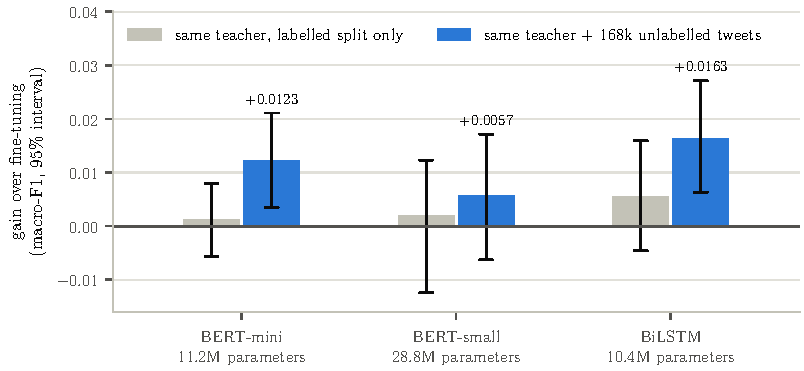
\includegraphics[width=\textwidth]{figures/fig_students.pdf}
\caption[The largest transfer set on three students]{Gain over fine-tuning from the same teacher, in sample and with 168,000 unlabelled tweets, on three students. Whiskers are paired bootstrap 95\% intervals.}
\label{fig:students}
\end{figure}

The BiLSTM gains most, every seed above every baseline seed, and at 10.4M parameters now clears the
classical floor (0.8798) and sits within 0.006 of DistilBERT's fine-tuning (0.8907) with a sixth of
the parameters. BERT-small gains on the mean, with two of three seeds above every fine-tuning seed,
but its fine-tuning seeds vary by 0.008 and its interval includes zero, which we report as it is. On
every student the gain lands in the same place: between fine-tuning and the 168k arm, F1 on
not\_cyberbullying rises from 0.644 to 0.671 on BERT-mini and from 0.690 to 0.734 on the BiLSTM, on
other\_cyberbullying from 0.707 to 0.720 and from 0.719 to 0.747, while the four targeted classes
move by at most 0.016. The unlabelled text teaches the boundary the labelled split draws worst.

The constructive sentence of this paper is therefore measured on four axes: the gain exists, it
grows with the unlabelled text, it comes from any tweets of the platform, and it holds on three
compact students of two families while fine-tuning for the same number of updates gains nothing.
What it does not have is a second corpus, which Chapter~\ref{ch:7} lists first.
\section{What Never Transferred: Discrimination of Implied Abuse Is Fixed by Pre-Training}
\label{sec:5.9}
\textbf{The failure is discrimination, not blindness.} Diagnostic on BERT-mini fine-tune-only, seed
1. Recall on the ironic-abuse probe is 0.91 on the 43 items containing explicit profanity and 0.76
on the 1,517 without; on the implicit-abuse probe 0.91 on 11 items with and 0.74 on 752 without.
Profanity helps, by 6 to 16 points of recall on every in-sample model analysed, but the items
without it are still caught about three times in four: the detector leans on profanity without being
a profanity detector. Mean $p(\text{abusive})$ is 0.748 on ironic abuse and 0.449 on benign sarcasm,
the distributions overlap heavily, and sarcasm-discrimination AUC is 0.773. At a 0.5 threshold,
recall of 0.792 costs a 39.5 per cent false-positive rate on sarcasm that attacks nobody. No
threshold up to 0.90 brings that rate under 10 per cent on any of the 29 in-sample models analysed;
three of the 14 out-of-sample and matched-steps models reach it at 0.90, at a recall of 0.31 to
0.39. The benchmark's own labels show the same confusion: other\_cyberbullying recall 0.710 with 109
of its errors going to not\_cyberbullying, and not\_cyberbullying recall 0.648 with 126 going the
other way.

\textbf{Nothing raises the discrimination} (Figure~\ref{fig:auc}). Over the 28 in-sample pre-trained
variants of BERT-mini analysed, which cover every objective and committee, seven temperatures, the
$T$, $\alpha$ and $\delta$ sweeps, every ablation and both controls, sarcasm-discrimination AUC has
mean 0.771 and standard deviation 0.004, from 0.756 to 0.777. The randomly initialised student
scores 0.613. The auxiliary irony head, the component built for this measurement, is inside the
band: without it 0.775, with it 0.773. Along the whole out-of-sample curve the first seed's AUC is
0.758, 0.764, 0.752, 0.765, 0.771 and 0.761, the generic control's 0.760, the 35-epoch control's
0.774 and the hard-label arm's 0.727: every pre-trained variant of the student lies between 0.72 and
0.78, and every soft-label variant between 0.75 and 0.78. This is where a pre-registered prediction
failed as written: the transfer run's predictions included the claim that the AUC would stay inside
the in-sample band of 0.756 to 0.777 on every arm, and three of the five arms fall below that band,
the hard-label arm furthest at 0.727. Nothing rises above it.

\begin{figure}[htbp]
\centering
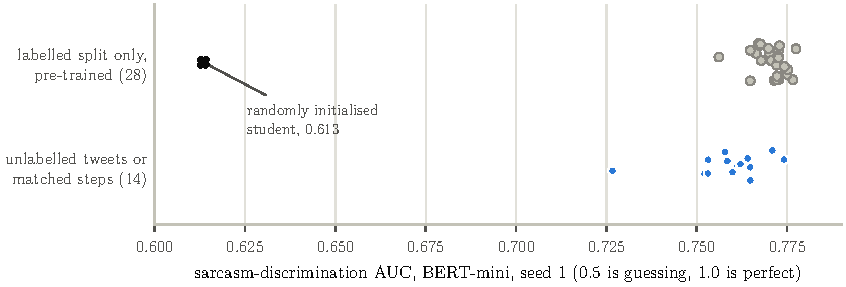
\includegraphics[width=\textwidth]{figures/fig_auc.pdf}
\caption[Sarcasm-discrimination AUC of every analysed variant]{Sarcasm-discrimination AUC of every analysed BERT-mini variant, first seed. Every pre-trained variant lies between 0.72 and 0.78, in sample or out; only removing pre-training moves the measure.}
\label{fig:auc}
\end{figure}

What moves is the operating point. Over the 28 pre-trained in-sample variants, recall at 0.5 ranges
from 0.758 to 0.821 and the false-positive rate from 0.343 to 0.448, correlated at +0.87; along the
out-of-sample curve both fall together, recall from 0.74 to 0.57 and the false-positive rate from
0.35 to 0.25 as the set grows to 168,000 rows, and on the BiLSTM to 0.50 and 0.18. The out-of-sample
student fires less on sarcasm of both kinds; it does not tell them apart any better.

\textbf{Across the grid, methods differ only in how readily they fire} (Figure~\ref{fig:tradeoff},
Table~\ref{tab:families}). Across all 184 evaluated models in the grid, teachers and students, every
mode and seed, the false-positive rate on benign sarcasm and the recall on ironic abuse correlate at
+0.772. Recall minus false-positive rate has mean 0.357 and standard deviation 0.046, while its
components range over 0.14 to 0.59 and 0.48 to 0.81. The 42 out-of-sample models do not leave the
curve, they slide along it: among themselves they correlate at +0.922, with the same mean margin,
0.355.

\begin{figure}[htbp]
\centering
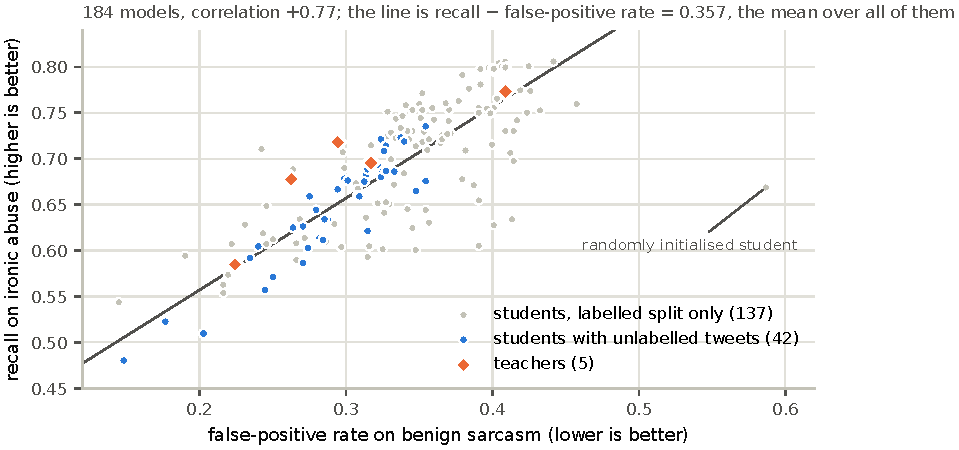
\includegraphics[width=\textwidth]{figures/fig_tradeoff.pdf}
\caption[False-positive rate against recall, all 184 models]{False-positive rate on benign sarcasm against recall on ironic abuse for all 184 evaluated models. Every family and objective lies along one trade-off line; the out-of-sample students slide along it rather than rising above it.}
\label{fig:tradeoff}
\end{figure}

\begin{table}[htbp]
\centering
\small
\caption[Probe metrics by model family]{Probe metrics by model family, averaged over all 184 evaluated models, at each model's argmax decision. The margin is recall minus false-positive rate.}
\label{tab:families}
\begin{adjustbox}{max width=\textwidth}
\begin{tabular}{lcccc}
\toprule
Model family & n & Benign FPR & Ironic recall & Margin \\
\midrule
DeBERTa-v3-xsmall & 21 & 0.334 & 0.728 & 0.394 \\
Teachers & 5 & 0.301 & 0.690 & 0.388 \\
DistilBERT & 21 & 0.238 & 0.607 & 0.369 \\
BERT-mini & 89 & 0.350 & 0.718 & 0.368 \\
BERT-small & 24 & 0.369 & 0.700 & 0.332 \\
BiLSTM & 24 & 0.316 & 0.608 & 0.292 \\
\bottomrule
\end{tabular}
\end{adjustbox}
\end{table}

Distillation mode does not appear in this ordering; architecture does. The models occupy different
points on one trade-off curve rather than different curves, and the worst margin in the grid, 0.082,
belongs to the randomly initialised student. Whatever ability these models have to tell implied
abuse from harmless sarcasm comes from pre-training, and nothing added to the objective or to the
data moves it. This is why the paper reports a threshold-free area: recall at a fixed cut measures
how readily a model fires, and across 184 models that is all it measures.

\textbf{The same failure on a corpus that labels implication} (Table~\ref{tab:implicit}).

\begin{table}[htbp]
\centering
\small
\caption{The implicit benchmark: the compact student, the specialist and the classical floor, one seed.}
\label{tab:implicit}
\begin{adjustbox}{max width=\textwidth}
\begin{tabular}{lccccc}
\toprule
Model & macro-F1 & not\_hate F1 & explicit\_hate F1 & implicit\_hate F1 & Implicit-discrimination AUC \\
\midrule
Classical floor & 0.5620 & -- & -- & 0.5562 & 0.7610 \\
BERT-mini, fine-tune only & 0.5549 & 0.8347 & 0.2857 & 0.5443 & 0.8196 \\
HateBERT specialist & 0.6029 & 0.8352 & 0.3662 & 0.6072 & 0.8247 \\
\bottomrule
\end{tabular}
\end{adjustbox}
\end{table}

The compact student loses to a bag of n-grams on F1 and beats it decisively on ranking: it separates
implied abuse from benign text at 0.8196 AUC against 0.7610 while scoring below the floor on the
implicit class itself. The two measures disagree in direction, not degree, which is the argument of
this section made on other people's labels. Both neural models score 0.29 to 0.37 on the 108-row
explicit class, which is why macro-F1 is not the headline here; these are single-seed results.
Applied without further training to the benchmark's 2,064 test posts, the tweet-trained BERT-mini
calls 81.0 per cent of them abusive against a true rate of 35.7 per cent (binary macro-F1 0.423,
ROC-AUC 0.608). On implicit hate against posts that are not hateful it catches 85.1 per cent at a
78.8 per cent false-positive rate. It ranks the two at an AUC of 0.600, barely above chance, against
0.820 for the same architecture trained on the corpus. D-MTHD transfers no better: binary macro-F1
0.411, the same two AUCs at 0.609 and 0.600. Whatever the tweet students have learned about abuse,
in sample or out, does not include what makes an implication hateful; there was little of that
knowledge in the committee to receive, and none in the transfer text.
\section{Character-Level Obfuscation and Deployment Cost}
\label{sec:5.10}
Table~\ref{tab:robustness} gives macro-F1 under synthetic obfuscation of the abusive test rows, on
BERT-mini, seed 1.

\begin{table}[htbp]
\centering
\small
\caption[Macro-F1 under character-level obfuscation]{Macro-F1 under synthetic character-level obfuscation of the abusive test rows: letters replaced by digits, adjacent characters swapped, spaces inserted, and all three together. BERT-mini, seed 1.}
\label{tab:robustness}
\begin{adjustbox}{max width=\textwidth}
\begin{tabular}{lccccc}
\toprule
Objective & Clean & Leetspeak & Character swap & Inserted spaces & Mixed \\
\midrule
Fine-tune only & 0.8394 & 0.7475 & 0.7417 & 0.7275 & 0.7116 \\
D-MTHD & 0.8385 & 0.7460 & 0.7361 & 0.7250 & 0.7077 \\
\bottomrule
\end{tabular}
\end{adjustbox}
\end{table}

Nine to thirteen points lost on short text, and distillation does not help: the two objectives are
within 0.006 of each other under every edit. These are character edits, not evasion by people trying
to evade, and we do not call the result robustness.

Table~\ref{tab:efficiency} gives the median of five timed passes after warm-up on an idle machine.

\begin{table}[htbp]
\centering
\small
\caption[Deployment profile of the students and the largest teacher]{Deployment profile of the students and the largest teacher: parameters, latency at batch sizes 1 and 32, FLOPs per sequence, model size, and macro-F1 after INT8 dynamic quantisation.}
\label{tab:efficiency}
\begin{adjustbox}{max width=\textwidth}
\begin{tabular}{lccccccc}
\toprule
Student & Params & Latency b1 & Latency b32 & GFLOPs/seq & fp32 size & INT8 size & INT8 macro-F1 \\
\midrule
BiLSTM & 10.4M & 2.57 ms & 0.18 ms & $\sim$0 & 40 MB & 32 MB & 0.8736 \\
BERT-mini & 11.2M & 3.47 ms & 0.37 ms & 0.87 & 43 MB & 33 MB & 0.8319 \\
BERT-small & 28.8M & 3.74 ms & 1.25 ms & 3.36 & 110 MB & 73 MB & 0.8448 \\
DistilBERT & 67.0M & 5.22 ms & 3.72 ms & 11.17 & 255 MB & 132 MB & 0.8931 \\
DeBERTa-v3-xsmall & 70.8M & 23.49 ms & 3.25 ms & 10.57 & 270 MB & 209 MB & 0.8765 \\
BERT-large (teacher) & 335.1M & 26.56 ms & 21.65 ms & 78.92 & 1,279 MB & -- & -- \\
\bottomrule
\end{tabular}
\end{adjustbox}
\end{table}

DistilBERT matches BERT-large at 5.0 times fewer parameters and 5.8 times lower batch-32 latency;
INT8 dynamic quantisation halves its size for 0.003 macro-F1. BERT-mini's size falls only from 43 to
33 MB because 7.8M of its 11.2M parameters are the embedding table, which dynamic quantisation does
not touch. The out-of-sample recipe adds nothing to inference: the transfer set is used once, in
training, and the deployed student is the same model.

\section{The Research Questions, Decided}
\label{sec:5.11}
The four questions of Section~\ref{sec:1.4} are decided here on the measurements above, under one rule
fixed before any of them was run: a difference counts only if its paired bootstrap interval excludes
zero, and on a test set of 4,326 posts that requires roughly 0.007 macro-F1 (Section~\ref{sec:4.7}).
Table~\ref{tab:rq} states each decision beside the evidence that carries it; the paragraphs below give
the numbers. Chapter~\ref{ch:6} takes up what the decisions mean.

\begin{table}[htbp]
\centering
\footnotesize
\caption[The four research questions and their decisions]{Each research question, the rule that decides
it, the measurement that decides it, and the decision.}
\label{tab:rq}
\begin{adjustbox}{max width=\textwidth}
\begin{tabular}{p{2.0cm}p{3.5cm}p{5.6cm}p{2.3cm}}
\toprule
Question & Decided by & Measurement & Decision \\
\midrule
RQ1: does the weighted committee beat no teacher at all, in sample? & Any interval excluding zero among
the in-sample distillation-against-fine-tuning comparisons & 27 such comparisons, none excludes zero;
best of six per student is $+0.0012$ to $+0.0071$, five intervals of five containing zero; weighting
minus averaging is $-0.0034$ to $+0.0000$, every interval containing zero & \textbf{No}
(Sections~\ref{sec:5.2}, \ref{sec:5.3}, \ref{sec:5.5}) \\
RQ2: what explains that? & The mechanism has to be measured, not argued & Teachers end training at loss
0.033 to 0.077 on the split the student is distilled on; weights 0.332 / 0.337 / 0.331 against a uniform
0.333, and 0.318 / 0.356 / 0.326 even at $\tau = 0.05$; pairwise $\kappa$ 0.889 to 0.962, all four
teachers right on 83.2 per cent of the test set and wrong together on 4.7 & \textbf{Memorised labels,
saturated weights, spent diversity} (Sections~\ref{sec:5.4}, \ref{sec:5.6}) \\
RQ3: does unlabelled text the teachers never saw help, and how? & Decision D20, written before the run:
the 168k arm gains at least 0.012 with the interval clear of zero and still rising & $+0.0123$ [$+0.0035$,
$+0.0211$] at 168,000 tweets, monotone over six sizes from $+0.0010$ at 5,000; generic text within
$+0.0017$ [$-0.0066$, $+0.0113$] of abuse-domain text at the same size; fine-tuning for the same updates
$-0.0013$ [$-0.0106$, $+0.0072$]; BiLSTM $+0.0163$ [$+0.0063$, $+0.0271$] & \textbf{Yes, and it is the
text} (Sections~\ref{sec:5.7}, \ref{sec:5.8}) \\
RQ4: does any of it improve the reading of implication? & A threshold-free AUC rising above the
in-sample band of 0.756 to 0.777 & 28 in-sample pre-trained variants, mean 0.771, standard deviation
0.004; out-of-sample arms 0.727 to 0.771, three below the band and none above; the randomly initialised
student 0.613; across 184 models recall and false-positive rate correlate at $+0.772$ & \textbf{No}
(Section~\ref{sec:5.9}) \\
\bottomrule
\end{tabular}
\end{adjustbox}
\end{table}

\textbf{RQ1 is decided against the method.} The grid makes 27 in-sample comparisons of a distilled
student against the same student fine-tuned without teachers, and no interval excludes zero. Taking the
best of six configurations per student, which flatters the method, gives $+0.0012$, $+0.0040$,
$+0.0068$, $+0.0040$ and $+0.0071$ macro-F1, all five intervals containing zero and all five below the
0.007 the test set can resolve. Per-instance weighting against uniform averaging gives $-0.0007$,
$-0.0034$, $+0.0000$, $-0.0029$ and $-0.0029$, and across a hundredfold range of $\tau$ the headline
student moves by 0.0007 and stays under fine-tuning at every value. Adding a teacher trained on labelled
implication changes it by $+0.0005$ [$-0.0059$, $+0.0064$] under averaging and $-0.0005$ [$-0.0069$,
$+0.0055$] under weighting. The answer is no at this resolution, and Section~\ref{sec:7.1} records that
an absence at this resolution is not a zero.

\textbf{RQ2 is decided by three measurements rather than by argument.} Four of the five teachers end
their last epoch at a cross-entropy between 0.033 and 0.077 on the split the weights are read from and
the student is distilled on, so their soft labels carry what the gold labels already carry; the one
teacher that did not memorise the split, DeBERTa at 0.227, is the one whose weight moves, to 0.233 in a
committee of four. The weights are therefore flat at every temperature the sweep reaches. And the
committee has little to route between: pairwise agreement runs from $\kappa = 0.889$ to $0.962$, the
four original teachers are right together on 83.2 per cent of the test set and wrong together on 4.7,
and no combination rule that sees only their probabilities, including a stacked gate fitted by
cross-validation on the test set, improves on their uniform mean by more than 0.005 against an oracle
sitting 4 to 5 accuracy points higher.

\textbf{RQ3 is decided for the data and against the committee.} Decision D20 fixed the rule before the
run: if the largest arm gained at least 0.012 with an interval clear of zero and the curve was still
rising, the constructive result would lead. It gained $+0.0123$ [$+0.0035$, $+0.0211$], the six sizes
are ordered without inversion from $+0.0010$ at 5,000 tweets, and the curve had not flattened. The three
controls hold: generic tweets of the same size come within $+0.0017$ [$-0.0066$, $+0.0113$] of
abuse-domain ones, fine-tuning for the same number of updates gains $-0.0013$ [$-0.0106$, $+0.0072$],
and the gain reappears on a second and third student, $+0.0163$ [$+0.0063$, $+0.0271$] on the BiLSTM and
$+0.0057$ [$-0.0063$, $+0.0171$] on BERT-small. The committee is not part of it: against a single
teacher on the same text it is $-0.0003$ [$-0.0061$, $+0.0056$], its corrected weighting adds $+0.0021$
[$-0.0017$, $+0.0082$], and its hard pseudo-labels gain $+0.0020$ against $+0.0070$ for its soft ones.

\textbf{RQ4 is decided against every intervention in the grid.} Measured without a threshold, 28
in-sample pre-trained variants of the headline student, covering every objective, committee,
temperature, sweep, ablation and control, have a sarcasm-discrimination AUC of mean 0.771 and standard
deviation 0.004. The out-of-sample arms run from 0.727 to 0.771: three of five fall below that band and
none rises above it, which is also where a pre-registered prediction failed as written. The only
intervention that moves the measure is removing pre-training, which drops it to 0.613. Across all 184
evaluated models recall on ironic abuse and the false-positive rate on benign sarcasm correlate at
$+0.772$ with a margin of $0.357 \pm 0.046$, so what the interventions change is where a model sits on
one trade-off line, not which line it is on. On a corpus that labels implication the same students rank
implied abuse against benign text at 0.600 to 0.609 AUC, against 0.820 for the same architecture trained
on that corpus.

\chapter{Discussion}
\label{ch:6}

\section{Answers to the Research Questions}
\label{sec:6.1}
\begin{description}
  \item[RQ1. Does multi-teacher distillation with per-instance weighting improve the compact student?]
    Not in sample. Across five students, three committees and every weighting temperature from 0.05 to 5,
    no distilled student beats the same student fine-tuned without teachers by more than the test set can
    resolve, and per-instance weighting never differs from uniform averaging (Sections~\ref{sec:5.2}
    and~\ref{sec:5.3}). A teacher trained on labelled implication changes nothing either
    (Section~\ref{sec:5.5}).
  \item[RQ2. Why not?] The student is distilled on the split the teachers were fine-tuned on, where they
    have memorised the labels. There their soft labels are the gold labels, the reliability signal that
    weights them is saturated, and task adaptation has made them agree on more than nine tweets in ten
    (Sections~\ref{sec:5.4} and~\ref{sec:5.6}).
  \item[RQ3. Does distillation on unlabelled text help, and on what does the gain depend?] Yes. On
    BERT-mini the gain grows monotonically with the amount of unlabelled text, from +0.0010 at 5,000
    tweets to +0.0123 [+0.0035, +0.0211] at 168,000. Generic tweets from the same platform work nearly as
    well as abuse-related ones, fine-tuning for the same number of updates gains nothing, and the gain
    holds on the BiLSTM (+0.0163) and on BERT-small (+0.0057, with an interval that includes zero). One
    teacher is enough: the committee, its weighting and hard pseudo-labels add nothing
    (Sections~\ref{sec:5.7} and~\ref{sec:5.8}).
  \item[RQ4. Does any of it improve the discrimination of implied abuse from harmless sarcasm?] No. Every
    pre-trained variant of the student, in sample or out, ranks ironic abuse above benign sarcasm with an
    AUC between 0.73 and 0.78. The interventions change how readily the student fires, not what it can
    tell apart (Section~\ref{sec:5.9}).
\end{description}

\section{What the Findings Mean}
\label{sec:6.2}

\textbf{What the audit says about error-weighted multi-teacher distillation.} The family's weighting
rule scores each teacher's reliability against the gold label on the training set. For teachers
fine-tuned on that set the score is saturated, and the weights it produces are uniform whatever the
temperature. Correcting the estimate, by scoring reliability out of sample as Section~\ref{sec:3.5}
does or by fitting a gate on held-out data, is necessary for the rule to mean anything, and on a
committee assembled in the usual way it is not sufficient: the teachers' outputs do not carry the
information needed to pick the right one where they disagree, so the reachable gain over uniform
averaging is a few tenths of a point, in sample and out. The five-point oracle gap is real, and it
is made of instances on which the teachers, and very likely the annotators, are uncertain.

\textbf{What it says about the committee.} Assembling specialists for complementary expertise and
then fine-tuning them on one corpus produces teachers that agree at kappa 0.9 and share their
errors. The adaptation cannot be skipped, because it is what makes the specialists' outputs
comparable; it can only be paid for. A committee that keeps its diversity needs at least one member
whose knowledge was not obtained by fitting the target training set. Out of sample, where the
committee does hold a better label than any of its members, the student still receives no more from
three teachers than from one: on this task a single large teacher's soft labels on unseen text are
the whole of what distillation transfers, and the cost of a committee is three times the caching for
nothing.

\textbf{What it says about where distillation's gain is.} In sample the teachers' soft labels are
the gold labels and distillation reduces to fine-tuning; out of sample they carry information the
gold labels do not, and a compact student receives it in proportion to how much such text it sees.
The recipes that report large gains for small students distil on transfer sets larger than the
labelled data \cite{tang2019distilling, jiao2020tinybert, turc2019wellread}, and Beyer et al.'s
account of distillation as function matching says why: a function is learned where it is sampled,
and sampling it only where it equals the label teaches the label \cite{beyer2022knowledge}. What our
measurements add is the domain-specific shape. The curve is monotone over a 34-fold range of size
and has not saturated at 168,000 rows; generic tweets carry most of the value, so the text need not
be abuse-related, only in the register the student will meet; the gain is not optimisation length,
which on its own overfits from the thirteenth epoch; and the heterogeneous student, which cannot
share the teacher's representation, gains most, which places the effect in the soft labels rather
than in the hidden-state term. The cost is one forward pass of one teacher over the unlabelled text
and a longer student run; the deployed model is unchanged.

\textbf{What it says about implication.} The gain lands on the two classes the labelled split draws
worst, not\_cyberbullying and other\_cyberbullying, and nowhere else. Recall at a fixed threshold
and the false-positive rate on harmless sarcasm move together across 184 models; a method that
reports only the first can claim progress on implication by lowering its threshold, and the
out-of-sample students do the opposite, firing less on sarcasm of both kinds while discriminating no
better. The threshold-free measure shows the ability to be fixed by pre-training and unmoved by
every objective, committee, teacher and transfer set we tried. If unlabelled text is to teach
implication, its composition is the variable, not its size: nothing in 205,593 tweets of offence and
sentiment carries the distinction the probes measure, and a transfer set that did would have to be
built from text in which implication is present and marked, which is the corpus of
Section~\ref{sec:4.2} and not the platform's ordinary stream.

\textbf{What it says about reporting.} Every out-of-sample result in this paper was predicted in
writing before the run that tested it, with thresholds and a decision rule, and scored by a script
against the generated tables; three of the eleven predictions failed as written and are reported as
such. A test set of 4,326 posts cannot resolve differences under 0.007 macro-F1, which is larger
than every in-sample distillation effect in the grid and than most differences reported in this
literature. The multi-teacher results the field has published for this task were obtained without
the fine-tuning control, the teachers' own scores, seeds or intervals; under those conditions our
in-sample grid would also have read as a success.

\section{How the Study Changed}
\label{sec:6.3}
The design of this thesis changed four times, and each change was forced by a measurement rather than
chosen in advance. Every change is recorded, with the evidence that forced it, in the decision log of
the project's repository.
\begin{enumerate}
  \item \textbf{From the Phase-2 method to a controlled grid.} The Pre-Thesis II report distilled two
    teachers into DistilBERT on the Wikipedia corpus and reported the student above its teachers from one
    run, without a student trained without teachers. On the cleaned tweet corpus we added that control,
    three seeds and paired bootstrap intervals, and distillation then raised every student by less than
    the test set can resolve.
  \item \textbf{From dynamic weighting to its mechanism.} The per-instance weights sat close to uniform at
    the default temperature and barely sharpened at a twentieth of it, and the score did not move.
    Measuring the teachers explained why: they had memorised the training split and agreed with one
    another on more than nine tweets in ten.
  \item \textbf{From a specialist teacher to the implication audit.} A teacher trained on labelled
    implication was added to supply the missing expertise. After task adaptation it behaved almost exactly
    like HateBERT, and no student became better at telling implied abuse from harmless sarcasm; the
    threshold-free measure showed that ability fixed by pre-training.
  \item \textbf{From the audit to out-of-sample distillation.} If the teachers' soft labels equal the gold
    labels on the training split, the lever is text the teachers have not fitted. Three runs, each with
    its predictions written down beforehand, then measured the gain, its growth with the amount of text,
    and its survival under the matched-compute and second-student controls.
\end{enumerate}
The title changed with the evidence. The registered title named a dynamic, multi-teacher, homogeneous
and robust framework. The grid measured each of those four properties and found none of them to be the
source of the gain, so the final title names what is.

\chapter{Limitations and Future Work}
\label{ch:7}
\section{Limitations}
\label{sec:7.1}
\textbf{One corpus.} Every claim about the out-of-sample curve rests on one benchmark, one platform
and one language. The Wikipedia grid and the student grid on the implicit benchmark were built and
not run within the compute available; the curve on DistilBERT and DeBERTa-v3-xsmall was not run
either. The claim is stated for compact students on this corpus, in the plural because it holds on
three students of two families, and for nothing wider.

\textbf{BERT-small's interval includes zero.} Its fine-tuning seeds vary by 0.008, and its
out-of-sample gain of +0.0057 sits inside that variance; the direction agrees with the other two
students and the per-class pattern is the same, but the number is a mean and is reported as one.

\textbf{Two machines disagree about the same configuration.} BERT-mini fine-tune-only scores 0.8779
on a laptop CPU and 0.8393 on a Kaggle T4 with identical code, data, seeds and hyper-parameters.
Mixed precision accounts for 0.0014 (full-precision Kaggle: 0.8407); the gold-label sequences match
row for row; re-running the current code on the laptop reproduces its result to sixteen significant
figures. The Kaggle run learns more slowly from the first epoch (training loss 1.02 against 0.87,
validation macro-F1 0.80 against 0.84), which points at the software stack, since the library
versions differ, rather than at the accelerator. Every table therefore comes from one environment
and comparisons are made only within it; the ranking of methods is unaffected because every run
shares the condition, and the discrimination AUC of the two environments' models differs by 0.003.
Absolute BERT-mini and BERT-small numbers may be under-trained by up to four points, which is also
why both sit below the classical floor in sample.

\textbf{Test-set size and seeds.} 4,326 test posts give paired intervals about 0.014 wide; three
seeds per main configuration and one for ablations, controls and sweeps. Differences are read from
intervals, not from seed variance, and single-seed rows are indicative only. The threshold-free
probe analysis covers the first seed of each configuration.

\textbf{The transfer set's provenance.} Its sources are public abusive-language and sentiment
corpora whose labels we discard; their texts were collected by other researchers under their own
sampling, and the generic portion is dominated by the emoji-prediction corpus. The screens against
every evaluation set are exact-match on normalised text; near-duplicates that differ by more than
punctuation, casing or mentions would pass them.

\textbf{Teacher variance is not estimated}; each teacher is trained once. \textbf{The heterogeneous
comparison is confounded}: DeBERTa-v3-xsmall is a weaker model on this task than the BERT-lineage
students, so the student swap mixes family with quality; the hidden-state term is the controlled
version of that question. \textbf{The probes are rule-built}, about 1,000 items each, with a
300-item human annotation in progress; probe metrics are reported only for models trained on
Twitter-domain data. \textbf{The label is contested}: the two corpora that annotate implication
agree on 48.2 per cent of shared hateful texts about whether the hate is implied, and every result
on that class is bounded by it. \textbf{Robustness} was measured with synthetic character edits.
\textbf{Distillation on an unlabelled transfer set is not new}; the contribution is the controlled
measurement in this domain, and a reader should not take the title's first clause as a method claim.

\section{Future Work}
\label{sec:7.2}
\begin{enumerate}
  \item \textbf{Transfer text that carries implication.} The out-of-sample gain is a task gain because
    nothing in the transfer text marks implication. Composing the transfer set from text in which implied
    abuse is present and labelled, such as the Implicit Hate Corpus used here as a benchmark, is the
    direct test of whether distillation can teach it.
  \item \textbf{A second corpus and the remaining students.} The Wikipedia personal-attacks pipeline is
    built and was not run within the compute available; the size curve on DistilBERT and
    DeBERTa-v3-xsmall was not run either.
  \item \textbf{Where the curve saturates.} The gain was still rising at 168,000 tweets. Larger transfer
    sets would locate its ceiling and its cost.
  \item \textbf{Human validation of the probes.} A 300-item annotation of sarcastic abuse by four
    annotators, with Fleiss' kappa, would replace rule-built probes with verified ones.
  \item \textbf{A teacher that keeps its diversity.} A committee member whose knowledge was not obtained
    by fitting the training split, such as a large language model used zero-shot, is the one committee
    for which per-instance reliability could have something to express.
  \item \textbf{Bengali.} The work was motivated by abuse in Bengali social media, for which no sarcasm
    teacher is available; the out-of-sample recipe needs only unlabelled text and one teacher, which makes
    it the natural first step there.
\end{enumerate}

\chapter{Conclusion}
\label{ch:8}
We built the multi-teacher distillation method the abusive-language literature keeps proposing, gave
it the teacher it was missing, and measured it under the controls it is rarely given.

In sample the method fails its own test. It does not beat a compact student trained with no teacher
on any of five students; its per-instance weighting does not differ from averaging at any
temperature; and a teacher trained on labelled implication adds nothing, in a committee, alone, or
as pre-training. The reason is measurable. The student is distilled on the split the teachers were
fine-tuned on, where they have memorised the labels, so their soft labels are the gold labels and
the reliability signal that weights them has nothing left to express.

Out of sample the same teacher earns its place. Its soft labels on unlabelled tweets raise the
headline 11M student by 0.012 macro-F1 at 168,000 tweets, with an interval clear of zero, and the
gain grows monotonically over six sizes. Generic tweets of the platform work nearly as well as
abuse-related ones. Fine-tuning alone for the same number of updates gains nothing. The 10M BiLSTM
gains 0.016, also clear of zero, and a 29M BERT gains 0.006 on the mean, with an interval that
includes it. At no point does the committee, its weighting or its hard pseudo-labels add anything to
what one teacher does.

What does not move is the part of the task the thesis set out to reach. Measured without a
threshold, the ability to tell implied abuse from harmless sarcasm is set by pre-training; no
objective, committee, teacher or transfer set we tried raises it, and recall at a fixed cut measures
only how readily a model fires. More unlabelled text helps, more teachers do not, and neither
teaches implication.

For practice, the recipe that survives is the oldest one in distillation, now measured in this
domain: one teacher, its soft labels on unlabelled text from the platform the student will serve,
screened against every evaluation set, and a compact student that is unchanged at inference. Two
caveats travel with it. The measurements run to 168,000 unlabelled tweets on one corpus in one
language, and the curve had not flattened there, so the ceiling is unknown. And the recipe buys its
gain by firing less: on the probes, recall on ironic abuse falls as the transfer set grows, which a
deployment must decide about knowingly.


\singlespacing
\bibliographystyle{unsrtnat}
\bibliography{references}

\appendix
\chapter{Pre-Registered Predictions and Their Outcomes}

\label{app:predictions}

Decisions D19, D20 and D21 in the repository's decision log state the predictions before each of the
three out-of-sample runs, and two of them also fix a decision rule for what the thesis would say
either way. \texttt{scripts/transfer\_verdict.py} and \texttt{scripts/scaling\_verdict.py} score
them against the generated tables. Of the eleven predictions, six held, two held in part (one of
their two clauses each), and three failed as written; both decision rules fired in favour of the
constructive framing. Prediction 10 was registered on means and is scored on means: BERT-small's
gain of +0.0057 has an interval that includes zero, which Section~\ref{sec:5.8} reports. The three
failures: the committee was predicted to be the better labeller for the student out of sample and
was not; the pre-registered committee arm was predicted to gain at least 0.010 and gained 0.007; and
the sarcasm-discrimination AUC was predicted to stay in its in-sample band on every out-of-sample
arm and fell below it on three of the five. All three failures are reported in
Sections~\ref{sec:5.7} to~\ref{sec:5.9}.

Table~\ref{tab:predictions} lists every prediction with the number that decided it. The session
column refers to Table~\ref{tab:sessions}.


{\footnotesize
\setlength{\tabcolsep}{4pt}
\begin{longtable}{p{0.8cm}p{0.9cm}p{7.0cm}p{3.6cm}p{1.2cm}}
\caption{Every prediction written before the out-of-sample runs, and its outcome.}
\label{tab:predictions}\\
\toprule
No. & Session & Prediction & Measured & Outcome \\
\midrule
\endfirsthead
\toprule
No. & Session & Prediction & Measured & Outcome \\
\midrule
\endhead
\bottomrule
\endfoot
1 & 5 & The committee with the transfer set beats fine-tuning by at least 0.010, interval excluding zero & +0.0070 [$-$0.0001, +0.0144] & failed \\
2 & 5 & The committee is a better labeller for the student than one teacher & $-$0.0003 [$-$0.0061, +0.0056] & failed \\
3 & 5 & Out-of-sample reliability weighting adds at most 0.003 over averaging & +0.0021 & held \\
4 & 5 & Hard pseudo-labels gain less than soft labels & +0.0020 against +0.0070 & held \\
5 & 5 & Sarcasm-discrimination AUC stays within 0.756 to 0.777 on every transfer arm & 0.727 to 0.765; three arms below & failed \\
6 & 6 & The gain rises with size at fixed composition, and 42k reproduces +0.006 to +0.009 & +0.0010, +0.0035, +0.0043, +0.0070 & held \\
7 & 6 & 42k generic tweets gain at least 0.003 less than 42k abuse-domain tweets, and generic rows beyond 42k add less per row & 0.0017 less; 0.4 against 1.7 per 10k & in part \\
8 & 6 & Fine-tuning for the 42k arm's updates gains at most 0.002, and the 42k arm beats it by at least 0.004 & +0.0027; +0.0043 & in part \\
rule & 6 & If the 168k arm gains at least 0.012 with the interval clear of zero and still rising, the constructive result leads & +0.0123 [+0.0035, +0.0211], rising & fired \\
9 & 7 & Fine-tuning for the 168k arm's updates gains at most 0.004, and the 168k arm keeps at least 0.006 over it with the interval clear of zero & $-$0.0013; +0.0136 [+0.0023, +0.0240] & held \\
10 & 7 & BERT-small's 168k arm gains at least 0.005 over fine-tuning and beats its in-sample single teacher & +0.0057; +0.0038, interval includes zero & held \\
11 & 7 & The BiLSTM's 168k arm gains at least 0.010 over fine-tuning & +0.0163 [+0.0063, +0.0271] & held \\
rule & 7 & If both controls hold, the result is stated for compact students in the plural & both held & fired \\
\end{longtable}
}


\chapter{Hyper-Parameters and Training Settings}
\label{app:hyper}
The distillation hyper-parameters ($\alpha = \beta = 0.4$, $\gamma = 0.2$, $\delta = 0.3$, $T = 4$,
$\tau = 1$) are carried over from the Phase-2 report's Table 3.1 unchanged, so that the audit tests
the method as proposed; Section~\ref{sec:5.3} sweeps each of them. Students train for 6 epochs at $3
\times 10^{-5}$ ($10^{-3}$ for the BiLSTM), batch 32, 10 per cent warm-up, linear decay, gradient
clipping at 1.0, early stopping with patience 2 on validation macro-F1; the matched-steps controls
disable early stopping and run 13 and 35 epochs. Teachers train for 5 epochs at $2 \times 10^{-5}$,
batch 32. Maximum sequence length 128.

\begin{table}[htbp]
\centering
\small
\caption{Training settings of the teachers and the students.}
\label{tab:hyper}
\begin{tabular}{p{3.6cm}p{4.2cm}p{5.8cm}}
\toprule
Setting & Teachers & Students \\
\midrule
Epochs & 5 & 6; 13 and 35 for the matched-steps controls \\
Learning rate & $2 \times 10^{-5}$ & $3 \times 10^{-5}$; $10^{-3}$ for the BiLSTM \\
Batch size & 32 & 32 \\
Schedule & 10\% warm-up, linear decay & 10\% warm-up, linear decay \\
Gradient clipping & 1.0 & 1.0 \\
Model selection & best validation macro-F1 epoch & best validation macro-F1 epoch; early stopping with patience 2, off for the matched-steps controls \\
Maximum length & 128 tokens & 128 tokens \\
Precision & mixed, on GPU & mixed, on GPU \\
Distillation & -- & $\alpha = \beta = 0.4$, $\gamma = 0.2$, $\delta = 0.3$, $T = 4$, $\tau = 1$ \\
Seeds & one run per teacher & 3; 1 for ablations, sweeps and controls \\
\bottomrule
\end{tabular}
\end{table}

\chapter{The Transfer Set}
\label{app:transfer}
\texttt{transfer\_report.json} and \texttt{transfer\_big\_report.json} record, for each source, the
rows read, the rows dropped as too short, as duplicates, and as overlapping each split, probe file
and implicit benchmark file, and the rows written. The base set of 42,013 rows is shuffled once with
seed 42; the extended set appends 163,580 generic rows after it, so that the size curve's arms are
the prefixes of one file.

\input{appendices/d_significance}
\chapter{Data and Reproducibility Statements}
\label{app:statements}
\textbf{Data.} English social-media text throughout; author demographics are not available and were
not inferred. Neither the implicit benchmark nor the transfer set is redistributed: no source is
ours to re-host. Both are released as build scripts plus per-row manifests (split, label or source,
SHA-1 of the normalised text) that let a reader verify a rebuild against ours without either party
redistributing text; the transfer-set reports record every count at every screen.

\textbf{Reproducibility.} Code, configuration, seeds and one-command drivers are public
(\url{https://github.com/mahdihasanshadi/THESIS}). Every reported number comes from a script that
writes a results file: the run tables and every interval are generated by \texttt{dmthd.tables} and
\texttt{dmthd.significance} from the saved per-run predictions, the teacher-combination table by
\texttt{scripts/committee\_rules.py}, and the probe analysis by \texttt{dmthd.implicit\_analysis}.
The decision log records every design decision with the evidence behind it and every pre-registered
prediction with its score, and the lab notebook records each run. Data preparation is deterministic
(seed 42) and reports every removal count. Checkpoints and cached teacher outputs are released with
the thesis. Compute: 18.4 GPU-hours on Kaggle T4 accelerators for the 179 runs of the tweet grid,
over the five sessions that ran to completion.

\end{document}
